\documentclass[a4paper]{article}


\usepackage[utf8]{inputenc}
\usepackage[affil-it]{authblk}
\usepackage[justification=centering]{caption}
\usepackage[numbers]{natbib}
\usepackage{amssymb}
\usepackage{color}
\usepackage{mathtools}


\newcommand{\red}[1]{\textcolor{red}{#1}}
\newcommand{\R}{{\mathbb{R}}}
\newcommand{\norm}[1]{\left\lVert #1 \right\rVert}
\newcommand{\overbar}[1]{
  \mkern 1.5mu\overline{\mkern-1.5mu#1\mkern-1.5mu}\mkern 1.5mu
}
\DeclareMathOperator*{\argmin}{arg\,min}
\DeclareMathOperator*{\argmax}{arg\,max}


\begin{document}


\title{Neural Machine Translation}
\author{Arul Selvam}
\author{Ehsan Nezhadian}
\affil{Rheinische Friedrich-Wilhelms-Universität Bonn}
\date{July 25, 2017}
\maketitle


\begin{abstract}
Machine translation (MT) is the task of automatically  translating  a  text from
one natural language into another. Ever since the invention of modern computers,
MT  has been  one of the  applications that envisioned  to be automated. In  the
recent years,the  progress in  MT has been  tremendous. In  today's mobile phone
era,  the need for MT systems is only  growing and  the demand  has grown beyond
just text  translation.  Live translation on video conferences  is possible with
the current MT systems. In this article, we discuss the  latest improvements  in
the MT research and highlight the most important breakthroughs.
\end{abstract}


\section{Deep Learning}

In  the  recent  years, Deep learning  has been  making  a big impact in various
fields of computer science. This impact is profound  in the  perceptual learning
task  in  the fields  like  computer  vision, natural  language  processing, etc
\cite{lecun2015deep}. Though the idea of training a multi layered neural network
to  perform function approximation is known to  the  research community  for  at
least  a  couple of  decades\cite{schmidhuber2015deep}, due  to  the  nature  of
training problem  requiring  large computational  resources,  the  multi layered
neural  network  remained less  practical. With  the advent  of general  purpose
graphical processing units (GPGPUs) and the  availability of training data,  the
neural networks are now a practical solution for many perceptual tasks.  One  of
the early success  of deep learning was in the field of image classification. In
the  annual ImageNet classification  challenge \cite{deng2009imagenet},  AlexNet
\cite{krizhevsky2012imagenet} showed a  remarkable improvement  in the state-of-
the-art accuracy. Within  a  few years,  more  sophisticated architectures  like
Google Inception  Network \cite{szegedy2016rethinking},  Deep  Residual  Network
\cite{he2016deep}, etc.,  have  improved the  accuracy  to be  comparable with a
human in that task. The generality of the neural network made it easily possible
to  be used  for  a wide  variety  of tasks.  With  more people working  on deep
learning  and  the   ideas  arising   in  solving   the  problems  being  easily
transferable, the deep learning is the state-of-the-art for many learning tasks.
In the following section, we will briefly summarize the basics of deep learning.


\begin{figure}
  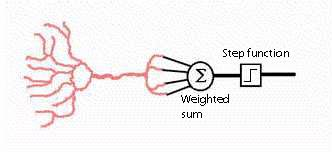
\includegraphics[width=.99\linewidth]{img/artificial.jpg}
  \caption{ An artificial neuron (perceptron)}
  \label{fig:ann}
\end{figure}


The basic  building block of a Multilayer  network,  or in  more  technical term
Multilayer  perceptron   (MLP)  is   a   perceptron.  The  preceptron  shown  in
Fig.\ref{fig:ann} closely  resembles  a  neuron in  a  human brain. A preceptron
takes a set of input values, computes a weighted sum of the  inputs, and outputs
a  scalar value  of a after applying an activation function (mostly non-linear).
The  weights for computing the weighted sum and the  threshold in the activation
function are initially  set to  random values  and are learned from the training
data. Mathematically, a  perceptron with the weight matrix $A$ and the threshold
$T$ for an  step activation  function, for  the  input vector  $x$,  outputs the
following,


\[
  f (x)=
  \begin{cases}
    1, & \text{if }  A x > c \\
    0, & \text{otherwise}
  \end{cases}
\]


A layer has many number of neurons and many layers are stacked one on top of the
other  to  form a MLP. An MLP  with many layers is called as Deep Neural Network
(DNN).  In the following section we  will discuss the properties of DNNs and how
they are useful in the context of supervised machine learning.


\begin{figure}
  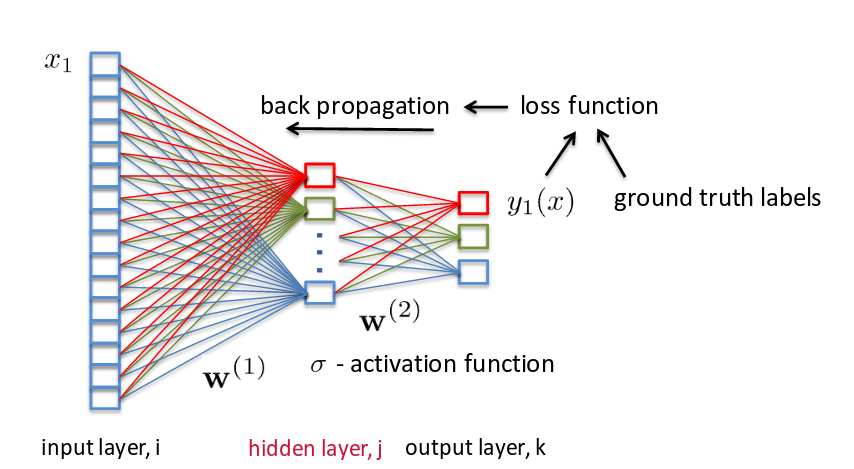
\includegraphics[width=.99\linewidth]{img/mlp.png}
  \caption{Layered representation in a MLP}
  \label{fig:mlp}
\end{figure}


\subsection{Supervised  learning}

Supervised  learning is the problem of predicting a new  output $y^\prime$ for a
new input $x^\prime$, and set of  training data that contains a set of input and
output  $\{x  \mapsto y\}$.  Most  of the supervised  learning problems  can  be
formulated as either a classification or  regression  problem. Classification is
the problem of predicting the label for a given $x^\prime$  among a set of given
labels $\{Y\}$, while  regression is predicting a continuous valued output for a
given input. The usual way of doing  supervised learning is to extract  features
from the given data and train a model to perform classification or regression.


\begin{equation*}
  x
  \xrightarrow[\text{Feature extraction}]{
    \mathbb{D}(x)
  }
  x^\prime
  _{intermediate}
  \xrightarrow[\text{classifier/regressor}]{
    \mathbb{F}(x^\prime | \theta)
  }
  y
\end{equation*}


The  power of  the DNNs  lies in  the  fact that  the models learns the features
directly from the given training data and avoids hand engineered features.


\begin{equation*}
  x \xrightarrow[ \text{hierarchical}] { \mathbb{M}(x | \Theta) } y
\end{equation*}


The DNNs with neurons in one  layers being  connected to all  the neurons in the
next  layer are called  Feed Forward Networks.  The  feed forward  networks  are
harder to  train since they have  lots of  parameters. To  make a the DNNs learn
useful representation for performing supervised learning, we need special  types
of  connections  between  the  neurons.  Two  of  the  most  commonly  used  DNN
architectures  are  Convolutional Neural  Networks  (CNN) and  Recurrent  Neural
Networks (RNN). In the following section we  will discuss these architectures in
detail.


\subsubsection{Convolutional Neural Networks}

Convolutional Neural netowrks  are  a class  of  feed-forward  networks in which
hidden  layers  are   either  convolutional,   pooling  for  fully-connected.  A
convolutional layer applies a convolution operation to the input, and passes the
result to  the next  layer. A pooling layer combines the outputs of  a number of
neurons from  previous  layer  into  a single value.  The  most common   pooling
operations are  max-pooling which selects the  maximum value from its  receptive
field  and  average-pooling which  calculates the  average  of values  from  its
receptive field.  A fully-connected layer  connects every neuron in one layer to
every neuron in another layer. Fig. \ref{fig:cnn} depicts a CNN.


\begin{figure}
  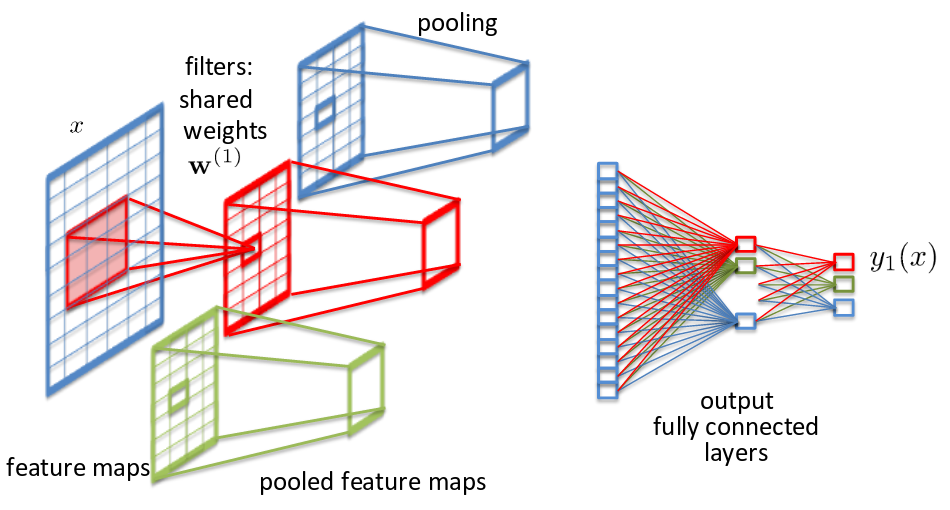
\includegraphics[width=.99\linewidth]{img/cnn.png}
  \caption{A CNN with a fully connected neurons in the last layer.}
  \label{fig:cnn}
\end{figure}


\subsubsection{Recurrent Neural Networks}

The neurons in the RNNs have recurrent self  connections. i.e. the output of the
neurons are connected back  to the inputs. Thus the output at time step $t_1$ is
computed with  taking  output  at  time  step  $t_0$  as  input.  The  recurrent
connections are  shown  Fig.\ref{fig:rnn}. This  enables  the  RNNs to  have  an
internal  memory.  RNNs  are  trained  with  the  a  modified  version  of  back
propagation   called    \textbf{Back    Propagation   Through    Time    (BPTT)}
\cite{werbos1990backpropagation}.

RNNs in general are harder to train and  this is particularity  evident when the
BPTT is  done over a larger number of time steps. This is because  the gradients
simply  converges  to  zero  after a  few time  steps.  This  problem  known  as
\textbf{vanishing   gradients   problem}   is   a   well    studied   phenomenon
\cite{bengio1994learning}.

To  alleviate  the  vanishing  gradients problem, a  special architecture called
\textbf{Long Short Term Memory (LSTM)} \cite{hochreiter1997long} is used.

LSTM cells has separate internal memory vector and has three gates--forget gate,
add gate, and output gate. To understand the Mathematical intuition behind these
gates, let  us consider a  LSTM  cell  in a hidden state  $h$  and internal cell
memory  vector $c_{t-1}$. At  time  $t$,  the  cell  takes input $x_t$, previous
output $h_{t-1}$ and update  the cell memory  to  $c_{t}$,  produces  the output
$h_{t}$. The forget  computes a  vector size $c$ between  0 and  1.  This vector
determines  what information should  be preserved and  what should be  forgotten
based on the current  input  $x_t$  as shown in  Fig.\ref{fig:lstm_forget}. This
vector is later  multiplied with the cell memory. If the vector  is  all  zeros,
multiplying makes all cell state to  forget  everything while  all ones preserve
everything. Then  the  add  gate computes which  parts in the  cell states to be
updates as shown  in Fig.\ref{fig:lstm_add} and the new  data  to  be updated as
shown in Fig.\ref{fig:lstm_add1}. Finally the  output gate generates  the output
$h_t$ and does not modify the cell state as shown in Fig.\ref{fig:lstm_output}.


\begin{figure}
  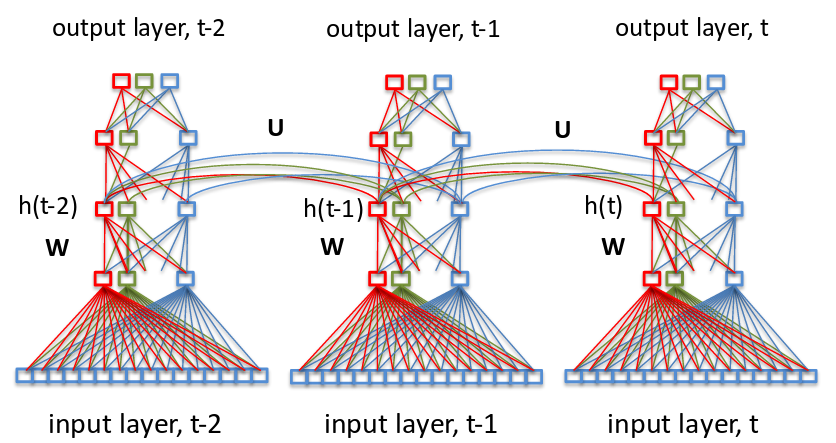
\includegraphics[width=.99\linewidth]{img/rnn.png}
  \caption{Recurrent connections in a RNN}
  \label{fig:rnn}
\end{figure}


\begin{figure}
  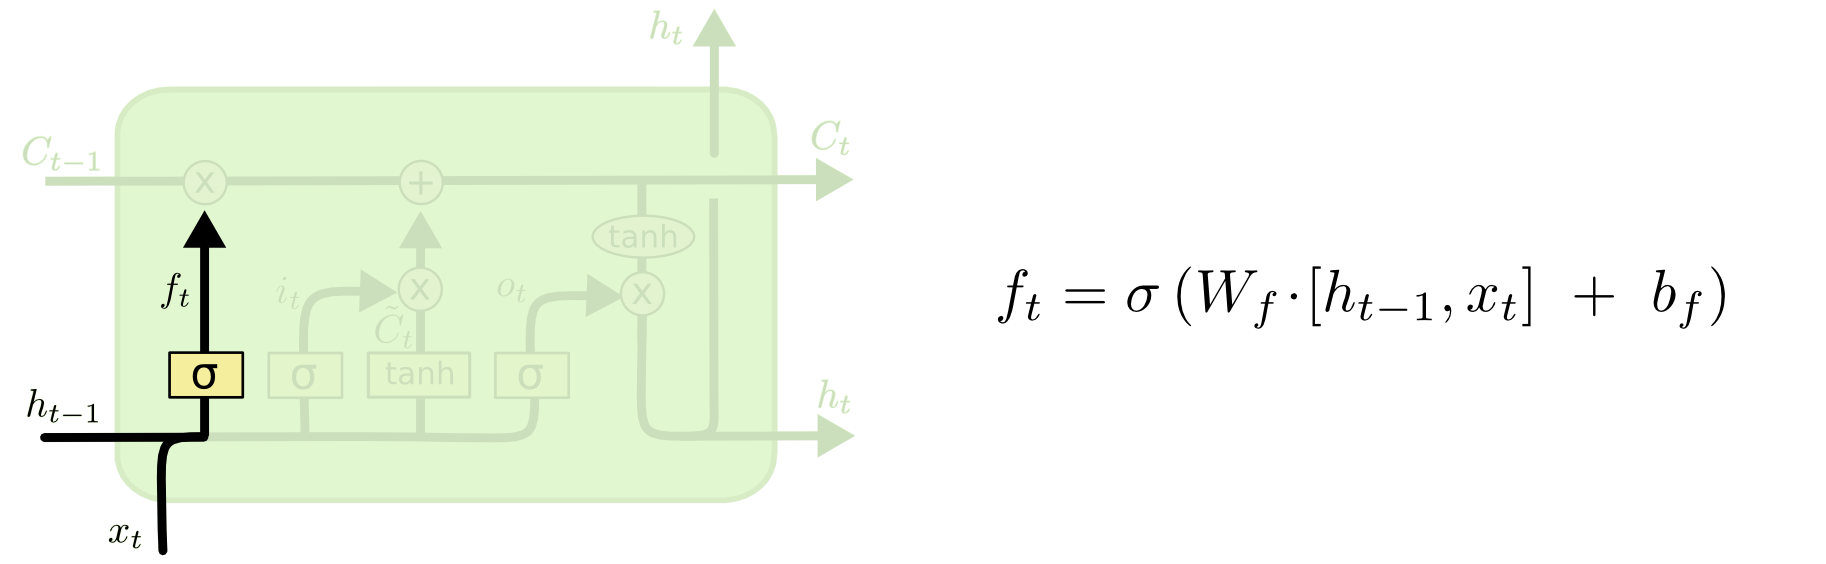
\includegraphics[width=.99\linewidth]{img/lstm_forget.png}
  \caption{Forget gate in LSTM}
  \label{fig:lstm_forget}
\end{figure}


\begin{figure}
  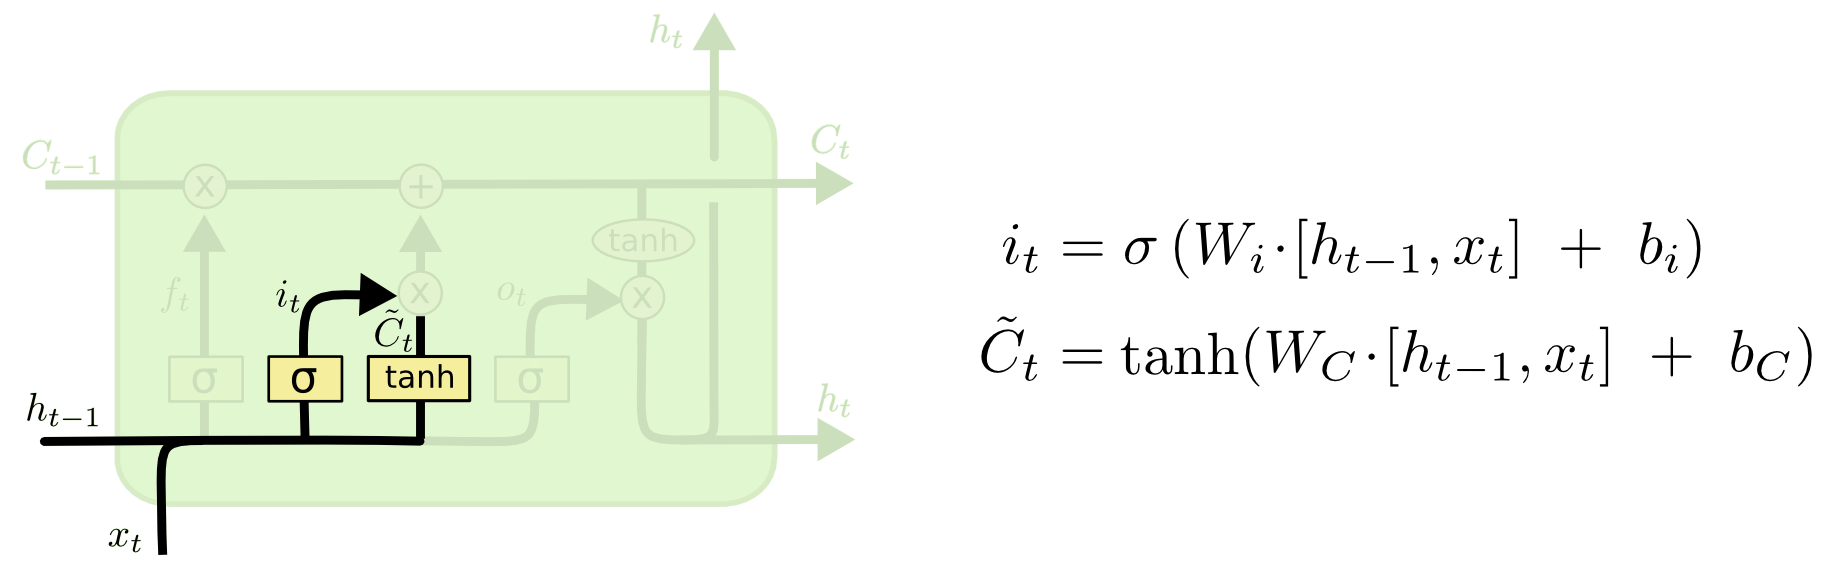
\includegraphics[width=.99\linewidth]{img/lstm_add.png}
  \caption{Add gate computing parts to be to modified in LSTM}
  \label{fig:lstm_add}
\end{figure}


\begin{figure}
  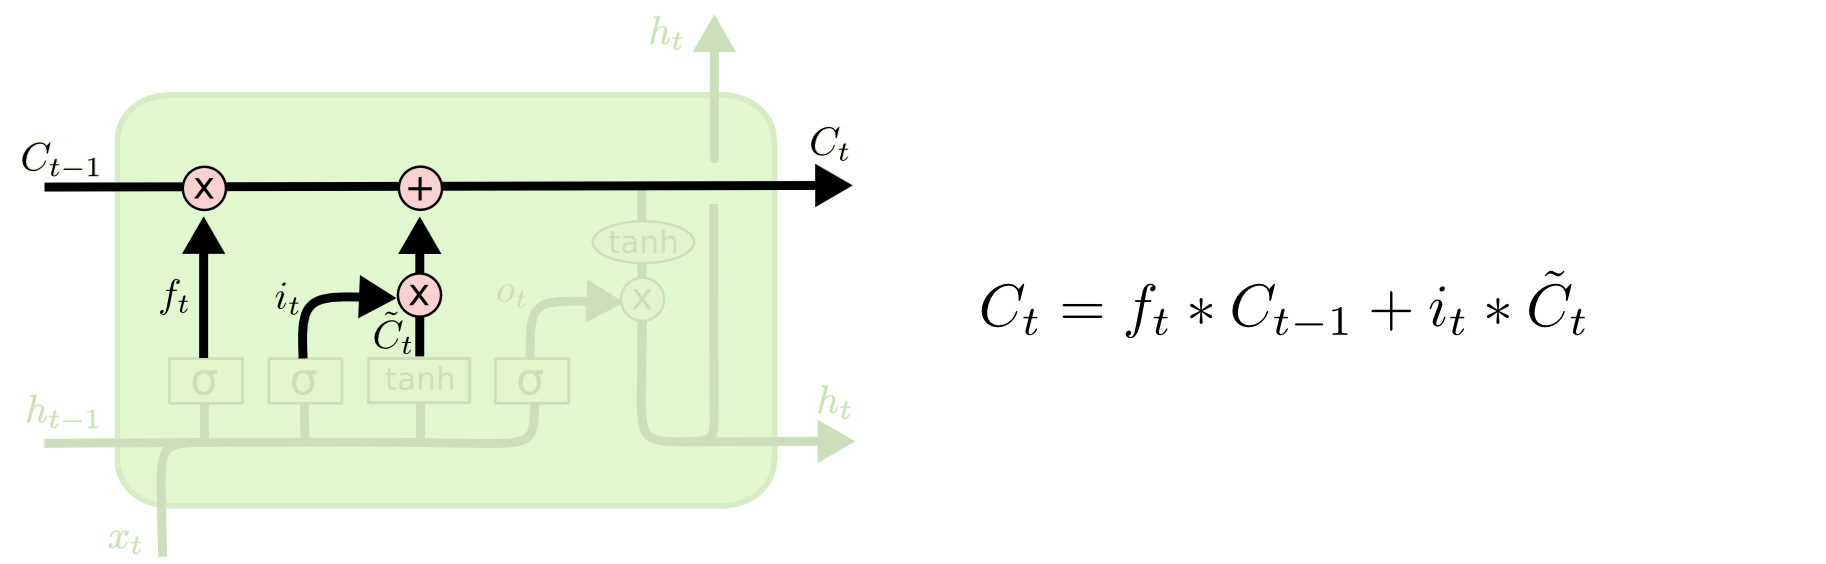
\includegraphics[width=.99\linewidth]{img/lstm_add1.png}
  \caption{Add gate computing data to be added to cell state in LSTM}
  \label{fig:lstm_add1}
\end{figure}


\begin{figure}
  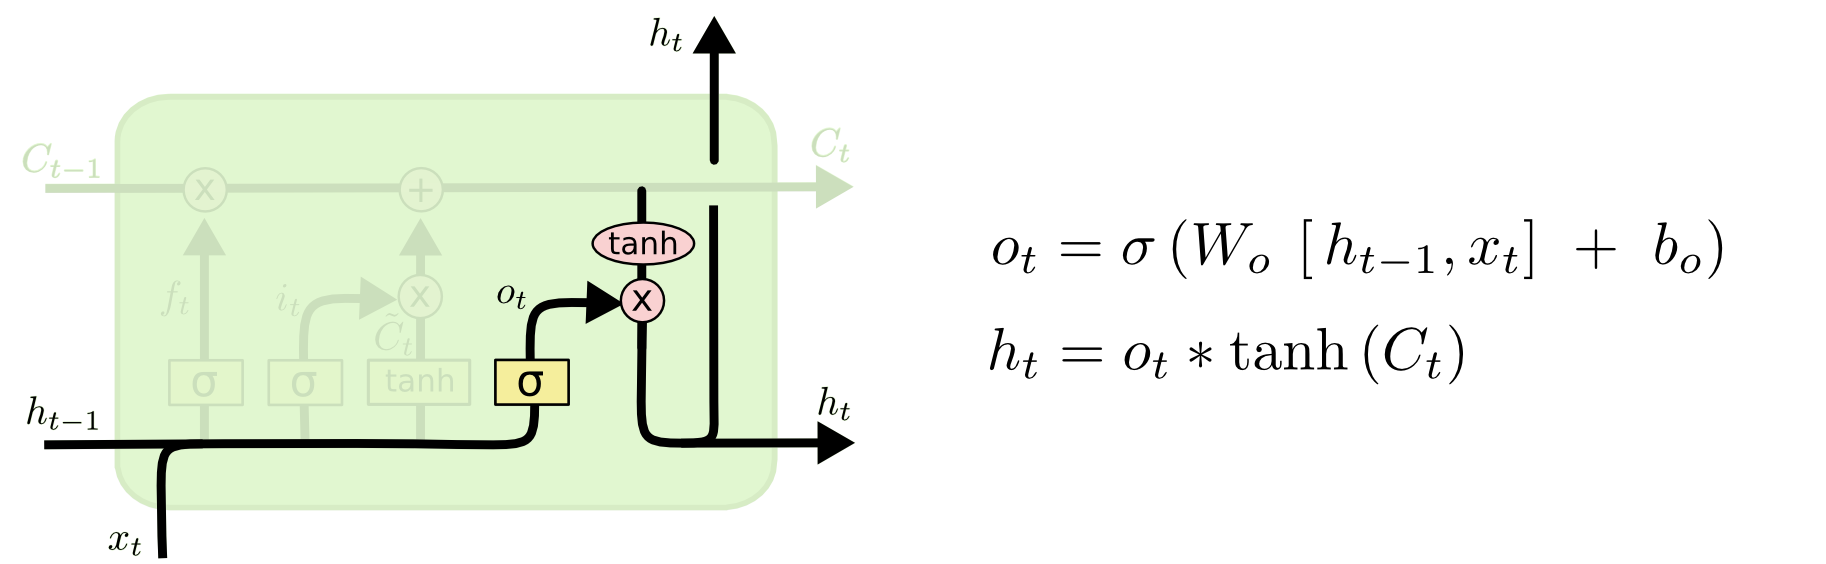
\includegraphics[width=.99\linewidth]{img/lstm_output.png}
  \caption{Add gate computing output in LSTM}
  \label{fig:lstm_output}
\end{figure}


\begin{figure}
  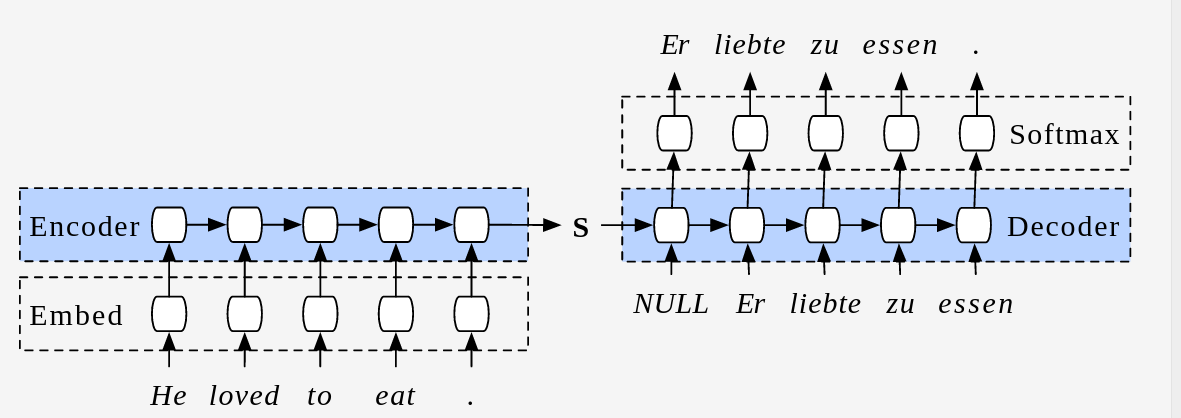
\includegraphics[width=.99\linewidth]{img/enc_dec.png}
  \caption{Simple Encoder-Decoder architecture for machine translation}
  \label{fig:enc_dec}
\end{figure}


\section{Traditional Machine Translation}

\subsection{Evaluation score}

Translation is a hard task to define an evaluation score for  measuring how well
a model is  performing  due to inherent complexity of the task. The most  widely
used  evaluation  metric  is  called  Bilingual   Evaluation  Understudy  (BLEU)
\cite{papineni2002bleu}.  It  depends  on  modified  n-gram  precision  (or  co-
occurrence) and needs lots of target sentences for better results. Despite being
the  most widely used metric, many researchers have expressed  concern about the
effectiveness of the metric \cite{zhang2004interpreting}, \cite{callison2006re},
\cite{ananthakrishnan2007some}. To understand how BLEU score works, consider the
following translation candidates


\begin{itemize}
  \item Candidate 1: It is  a  guide to action which ensures that  the  military
        always obey  the commands the  party.
  \item Candidate 2: It is  toinsure the troops  forever  hearing  the  activity
        guidebook that party  direct.
\end{itemize}


to be evaluated against the set of three reference translations.


\begin{itemize}
  \item Reference 1: It is a guide to action that ensures that the military will
        forever heed Party commands.
  \item Reference 2: It is the  guiding  principle which guarantees the military
        forces always being under the command of the Party.
  \item Reference 3: It  is  the  practical  guide  for  the army always to heed
        directions of the party.
\end{itemize}


The  BLUEs core idea is to use  count the  number  of N-gram  matches. The match
could  be position-independent. Reference could be matched multiple times. These
steps are linguistically-motivated.

Candidate  1:  \red{It is  a  guide to action which  ensures  that  the military
always} obey \red{the commands of the party}. \\
Reference 1: \red{It is a guide  to action} that \red{ensures that the military}
will forever heed \red{Party commands}. \\
Reference  2:  It  is  the  guiding principle  \red{which}  guarantees \red{the}
military forces \red{always}  being under  \red{the} command \red{of} the Party.
\\
Reference 3: It is the practical guide for the army always to heed directions of
the party. \\
N-gram Precision: 17

Candidate 2: \red{It is to} insure \red {the} troops \red {forever} hearing \red
{the} activity guidebook \red{that party} direct. \\
Reference 1: \red {It is} a guide \red {to} action \red {that} ensures that \red
{the} military will  \red{forever} heed \red{Party} commands. \\ Reference 2: It
is \red{the} guiding principle which guarantees the
military forces always being under the command of the Party. \\ Reference 3:  It
is the practical guide for the army always to heed directions of the party. \\
N-gram Precision: 8

Thus candidate 1 is better.

\textbf{Issues with N-gram precision:}

Candidate: \red{the the the the the the the.} \\
Reference 1: \red{The} cat is on the mat. \\
Reference 2: There is a cat on the mat. \\

\textbf{\red{N-gram Precision: 7 and BLEU: 1}}

This result is  very misleading. Thus the following modified BLEU score is often
used.


\begin{table}[h]
  \centering
  \begin{tabular}{ll}
    \hline
    \textbf{Algorithm}  & \textbf{Example}  \\
    \hline
    Count the max number of times & Ref 1: The cat is on the mat.  \\
    a word occurs in any single reference & Ref 2: There is a cat on the mat. \\
    & “the” has max count 2 \\
    \hline
    Clip the total count of & Unigram count = 7 \\
    each candidate word & Clipped unigram count = 2 \\
    &Total no. of counts = 7 \\
    \hline
    Modified N-gram & Modified-ngram precision: \\
    Precision equal to & Clipped count = 2 \\
    Clipped count/ & Total no. of counts =7 \\
    Total no. of candidate word & Modified-ngram precision = 2/7\\
    \hline
  \end{tabular}
  \caption{Translation evalution scores}
\end{table}


N-grams with different Ns are used but 4 is most common metric.


\subsection{Phrase based Machine Translation (PBMT)}

Traditionally there exists two types of machine translation systems:

\begin{itemize}

  \item \textbf{The Rule-based Approach}
        The  source language text is analyzed using parsers and/or morphological
        tools   and   transformed  into    intermediary   representation.   This
        representation  is  used  to  generate  target  sentence.  The rules are
        written  by human  experts. As  a large number of  rules is  required to
        capture  the  phenomena  of natural language,  this is a  time consuming
        process.  As the set of rules grows over time, it gets more and more
        complicated to extend it and ensure consistency.

  \item \textbf{The Data-driven Approach}
        In the data-driven  approach, bilingual and monolingual corpora are used
        as main knowledge source.  In the statistical approach, MT is treated as
        a  decision problem:  given the  source  language  sentence,  we have to
        decide  for the  target language  sentence that is the best translation.
        Then,  Bayes rule  and  statistical  decision theory are used to address
        this decision problem.
\end{itemize}


For a given sentence in source language $f^{I} = f_1\ldots f_i\ldots f_{I} $, we
need to find the sentence $e^{I} = e_1\ldots e_i\ldots e_{I}$ in target sentence
by applying Bayes rule to find the sentence that minimizes the expected loss


\begin{equation*}
e^{I} =  \argmin_{I,e^{I}} \Bigg\{
  \sum_{I^{'} } Pr(e^{\prime i^\prime} | f^J) \cdot L(e^I, e^{\prime i^\prime})
\Bigg\}
\end{equation*}


Here $L (e^I, e^{\prime i^\prime})$ denotes loss function under construction. It
measures  the loss  (or errors) of a candidate translation $e^{I}$ assuming  the
correct translation is $e^{\prime i^\prime}$. If the loss function is assumed to
be  0-1 loss meaning zero  if wrong and 1 if correct, then the Bayes rule can be
simplified to,


\begin{equation*}
  e^{I} = \argmax_{I,e^{I}} \Bigg\{Pr (e^{\prime i^\prime} | f^J) \Bigg\}
\end{equation*}


PBMT  were  the widely  scalable models  in  the  beginning  of  the  millennium
\cite{koehn2003statistical}. The model works  at the level of phrases instead of
words and  had  a lot of individual components  but  the  core idea is  learning
statistical patterns in training data.

Some of the major components used in the PBMT were


\begin{itemize}
  \item Sentence  alignment:   Gale   and  Church  Algorithm  based  on  Dynamic
        programming \cite{lewis1994sequential}.
  \item Word alignment: Expectation Maximization.
  \item Phrases generation: Heuristic based complex algorithms.
  \item Phrase lookup: Statistical matching.
  \item Beam search:  For  generating target sentence.  Beam search is a generic
        algorithm that is used even in the latest NMT systems.
\end{itemize}


Beam search in general is a heuristic search  algorithm that explores a graph by
expanding the most promising node in a limited set. In machine translation, beam
search is used to generate  a set of most likely sentence given a input sentence
by retaining  only the most promising  translations. Number of sentence  is kept
constant.


\section{Neural Machine Translation (NMT)}

Though usage of  neural networks did  not  yield  promising results in the early
years, the recurrent neural networks started to  achieve  performance comparable
to       PBMT       as       in       \cite{kalchbrenner2013recurrent}       and
\cite{hermann2013multilingual}. Most  of  the  early architectures  were  simple
encoder-decoder architectures. An simple working of encoder-decoder architecture
for machine translation is shown in Fig. \ref{fig:enc_dec}. The architecture has
an encoder that takes a sentence in source language and encodes it into a vector
$S$ of fixed length. The decoder takes the embedding $S$ as  input and generates
the sentence in the target language. Some of the major drawbacks with the simple
architecture is that


\begin{enumerate}
  \item The  encoder  has to  encode all the  information in the source sentence
        into fixed size embedding $S$.
  \item The decoder  never  sees  the  actual  input  sentence  and  has to rely
        completely on $S$ for generating target sentence.
  \item Having fixed size embedding vector makes the architecture less flexible.
        Smaller size means less  information where  as using larger vector means
        for smaller sentences we need zero padding and more computation time.
\end{enumerate}


\begin{figure}
  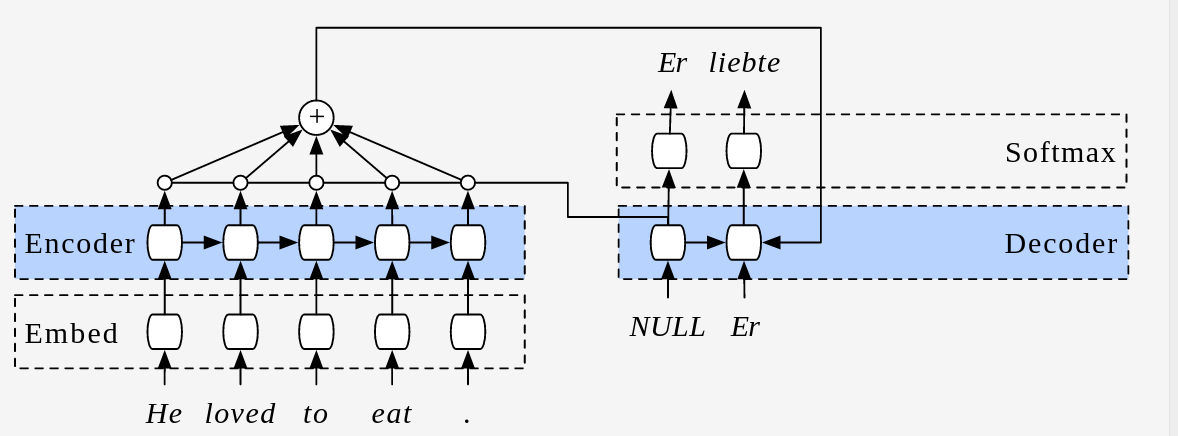
\includegraphics[width=.99\linewidth]{img/context.png}
  \caption{Context for machine translation}
  \label{fig:context}
\end{figure}


\subsection{Jointly learning to align and translate} \label{sec:JT}

The paper  \cite{bahdanau2014neural} address this issue  of having a  fixed size
embedding by introducing the idea of context  as shown in Fig.\ref{fig:context}.
The main proposal was


\begin{enumerate}
  \item Encoder  outputs a  hidden  representation  for  each word in the source
        sentence $F_s$.
  \item One context vector $C$ in the size of the input sentence that has values
        between 0 and 1.
  \item Each element of the embedding  $F_s$  is multiplied with one  element in
        $C$.
\end{enumerate}


The whole embedding is  made available to  the decoder  and $C$  describes which
part of  the embedding should be focused to generate  the current word based  on
the previous word.

Encoder  RNN  at  each  input  step t, generates hidden  state,  $h_t  =  f(x_t,
h_{t-1})$.  Unlike  in the previous models where  only the last hidden state  is
made available to the decoder, this paper provided all the hidden state and also
a  context vector that has a weight for each of the  hidden vector. The  context
vector  helps   the  decoder  to  focus  on  a  part  of  the  sentence.  $c   =
q(\{h_1,\cdots,h_{T_x}\})$.


The decoder is trained to predict the next work $y_t$  given the context  vector
$c$ and all previously predicted words $\{ y_1, \cdots, y_{t-1}\}$


\begin{equation*}
  p(y) = \prod^{T}_{t=1} p(y_t | \{ y_1, \cdots, y_{t-1}\}, c)
\end{equation*}


With RNN, each conditional probability is modeled as,


\begin{equation*}
  p(y_t | \{ y_1, \cdots, y_{t-1}\}, c) = g(y_{t-1}, s_t, c)
\end{equation*}


where  $s_t$ is the hidden  state  of  the RNN. The context vector  for a  input
sentence $i$, is  computed  as  a weighted  sum of  hidden states of the encoder
(also known as \textbf{annotations})


\begin{equation*}
  c_i = \sum_{j=1}^{T_{x}} \alpha_{ij} h_j
\end{equation*}


\begin{equation*}
  \alpha_{ij} = \frac{ exp (e_{ij})}{ \sum_{k=1}^{T_x} exp(e_{ik})}
\end{equation*}


where, $$ e_{ij}  = a(s_{i-1},  h_j)  $$ is the alignment model that  scores how
well the inputs around the $j$ and the output at the position $i$ match.

A   feedforward  neural  network   is  used  as   the  alignment  model  and  is
\textbf{jointly trained} with all the NMT system as a whole.


\begin{figure}
  \center
  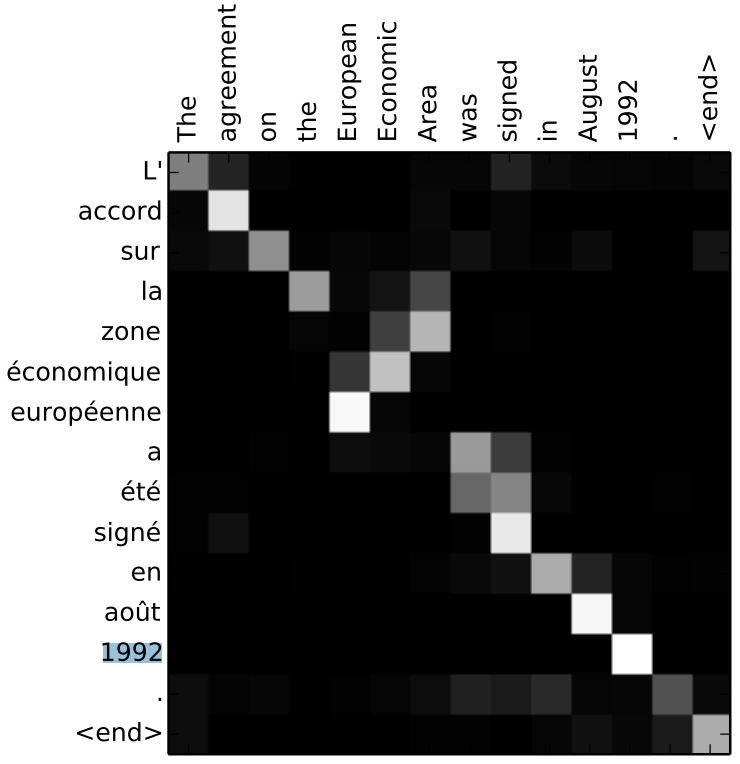
\includegraphics[height=8cm]{img/contextres.png}
  \caption{Visualization of the context in action}
  \label{fig:contextvis}
\end{figure}


The  functionality   of  the   context   vector  is  visualized  in   the   Fig.
\ref{fig:contextvis}.   For  example,  the  French  language   has   the   words
\textquotedblleft European Economic Area\textquotedblright exists in the reverse
order as \textquotedblleft zone \'{e}conomique europ\'{e}enne\textquotedblright.
The context learns to focus on the correct order for the decoder.

The idea of  context used in the paper was adapted by the MT  research community
with   the  name  of  attention.  Several  attention  mechanism   were  proposed
\cite{luong2015effective},  \cite{cho2014learning},  \cite{gregor2015draw}.  The
context proposed in section \ref{sec:JT} to  align hidden state  $h_t$ with each
source hidden state $\bar{h_s}$ can be formulated a,


\begin{equation}
  \begin{split}
    a_t(s) & = align(h_t,\bar{h_s}) \\
    & = \frac{exp(score(h_t,\bar{h_s}))}{\sum_{s'} exp(score(h_t,\bar{h_s'}))}
  \end{split}
\end{equation}


The new attention mechanisms proposed are,


\begin{equation*}
  align(h_t,\bar{h_s}) = \begin{cases}
    h_t^T\bar{h_s} & \text{dot} \\
    h_t^TW_a\bar{h_s} & \text{general} \\
    v_a^T tanh(W_a[h_t;\bar{h_s'}]) & \text{concat}
  \end{cases}
\end{equation*}


These mechanisms  are shown  do perform better  in certain scenarios but none of
them is shown to be the best.


\begin{figure}
  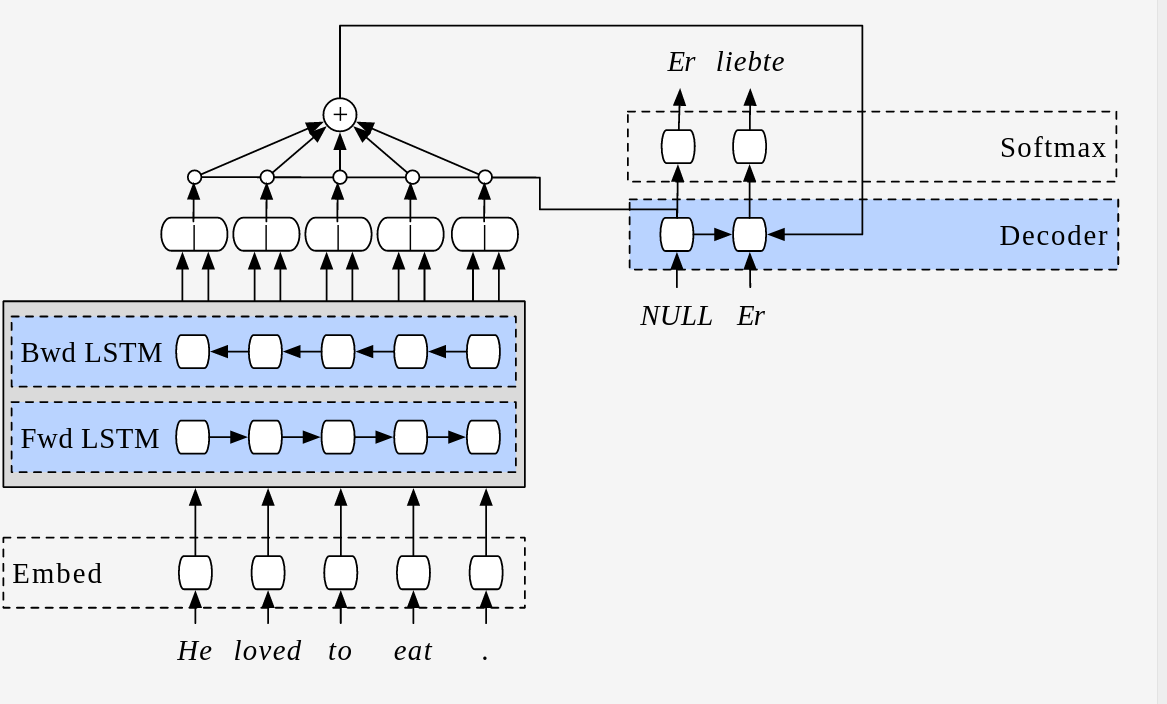
\includegraphics[width=0.9\linewidth]{img/birnn.png}
  \caption{Bi-directional Encoder}
  \label{fig:birnn}
\end{figure}


This paper  also made  use of  the  bi-directional  LSTM  in  the layers  of the
Encoder. Just like  an  LSTM that has an internal memory to comprehend  the past
states, the LSTM also comprehends the words that comes next in the sentence.  It
has two internal state---one for past states and one for the future state. A bi-
directional LSTM is shown in Fig.\ref{fig:birnn}.

The whole model is trained with standard maximum-likelihood  error  minimization
$\mathbb{O}_{ML}(\Theta) = \sum_{i=1}^N log P_\Theta(Y^{*(i)} |  X^{(i)}) $ with
stochastic gradient descent (SGD) on a mini-batch of 80 sentences. For the first
time, the BLEU score was comparable to phrase based machine  translation system.
But  the fact  that there  are  no  individual pieces  in the  model was a great
benefit and the  research  community started to  consider  neural systems as  an
viable alternative phrase based machine translation system.


\subsection{Sequence  to Sequence models}

\label{sec:seq}  With  in  an  year,  more   deep   and   powerful  models  were
computationally possible. Taking the availability of the computational power  to
advantage  a  new  framework  for  learning  sequence  to sequence  learing was
proposed. A sequence to sequence model formulated as $$ p(y_1, \cdots, y_T| x_1,
\cdots, x_T) =  \prod_{t=1}^{T} p(y_t| v, y_1,  \cdots,  y_{t-1})$$ where $v$ is
the internal memory of the RNNs. With more powerful RNNs, this model can be used
to  learn a  variety  of  tasks  like  speech  recognition,  handwritten  digits
recognition,   machine   translation,    etc    as   shown    in    the    paper
\cite{sutskever2014sequence}


\begin{figure}
  \centering
  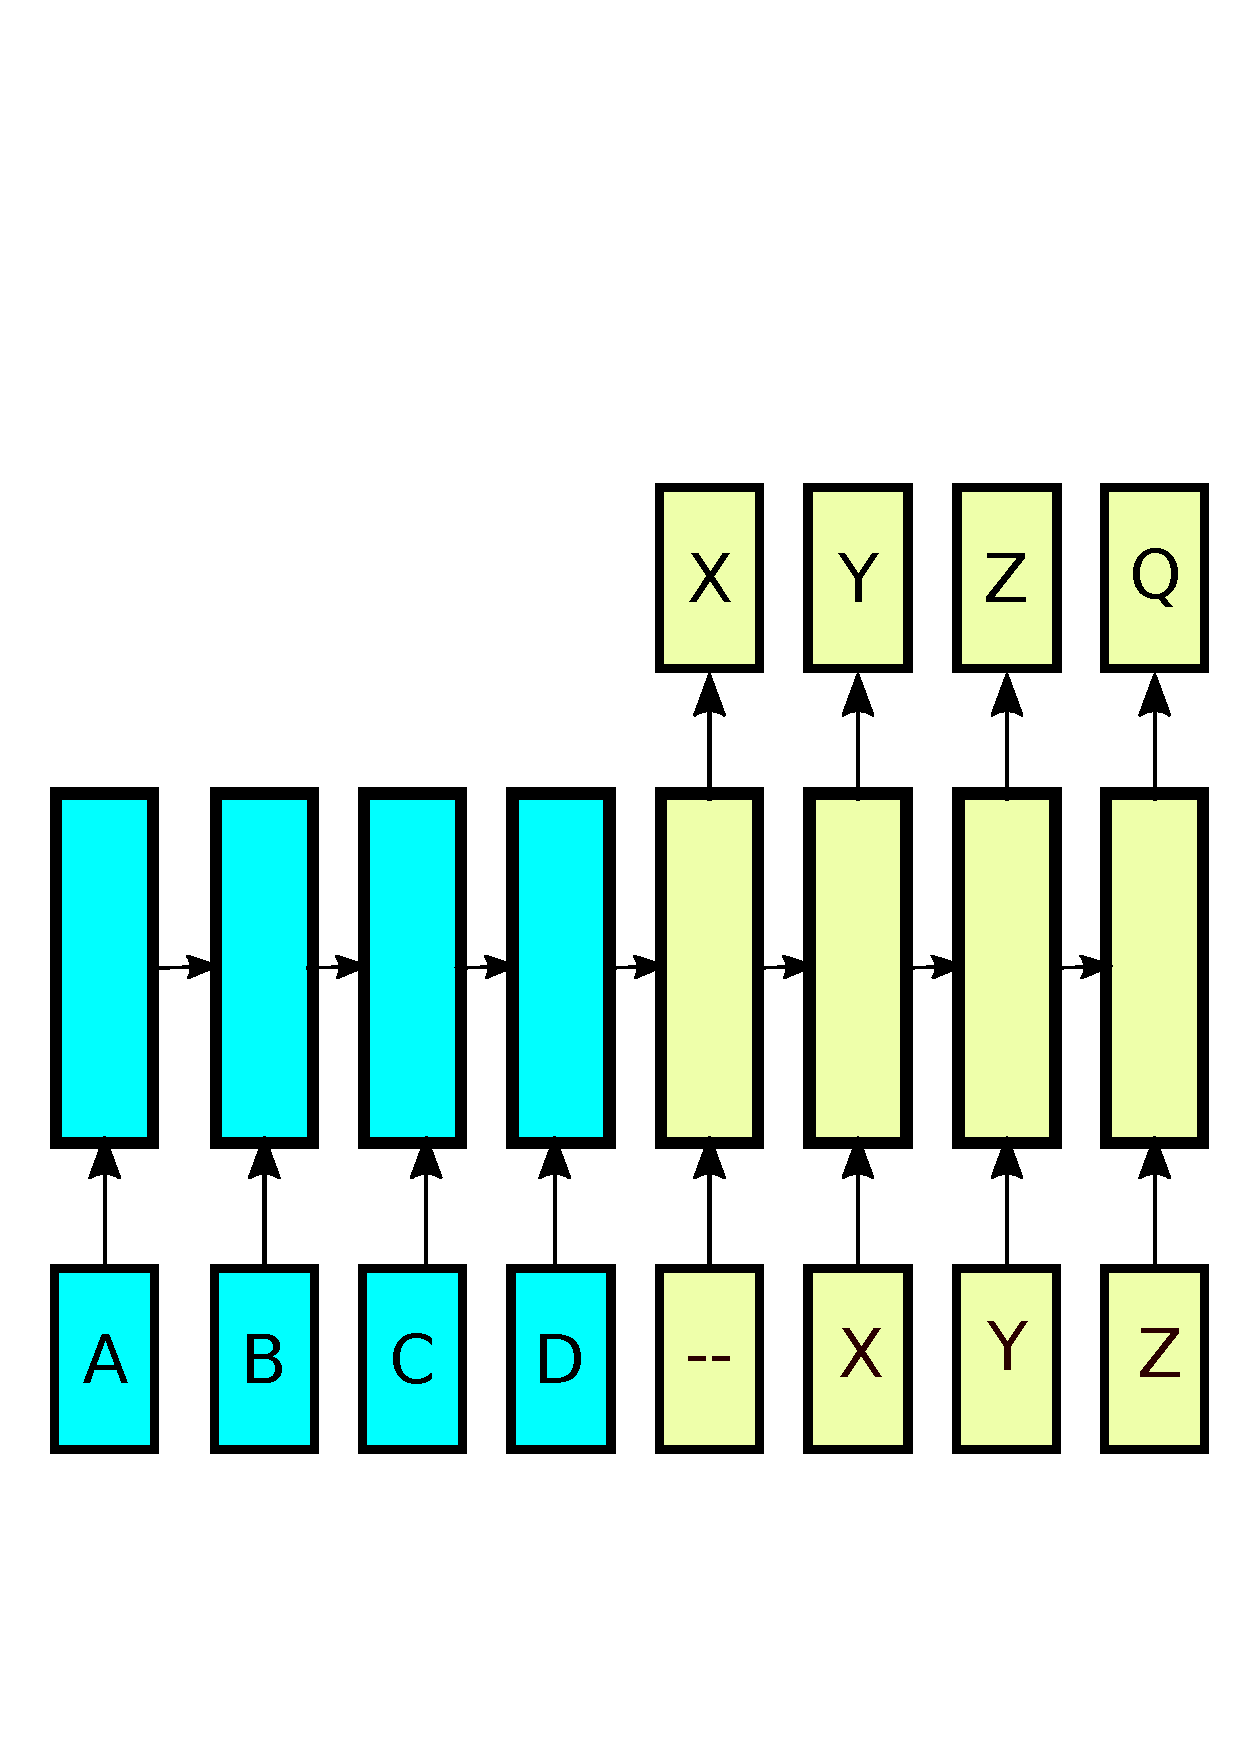
\includegraphics[width=.49\linewidth]{img/seq2seq.pdf}
  \caption{Sequence to sequence model}
  \label{fig:seq}
\end{figure}


\begin{figure}
  \centering
  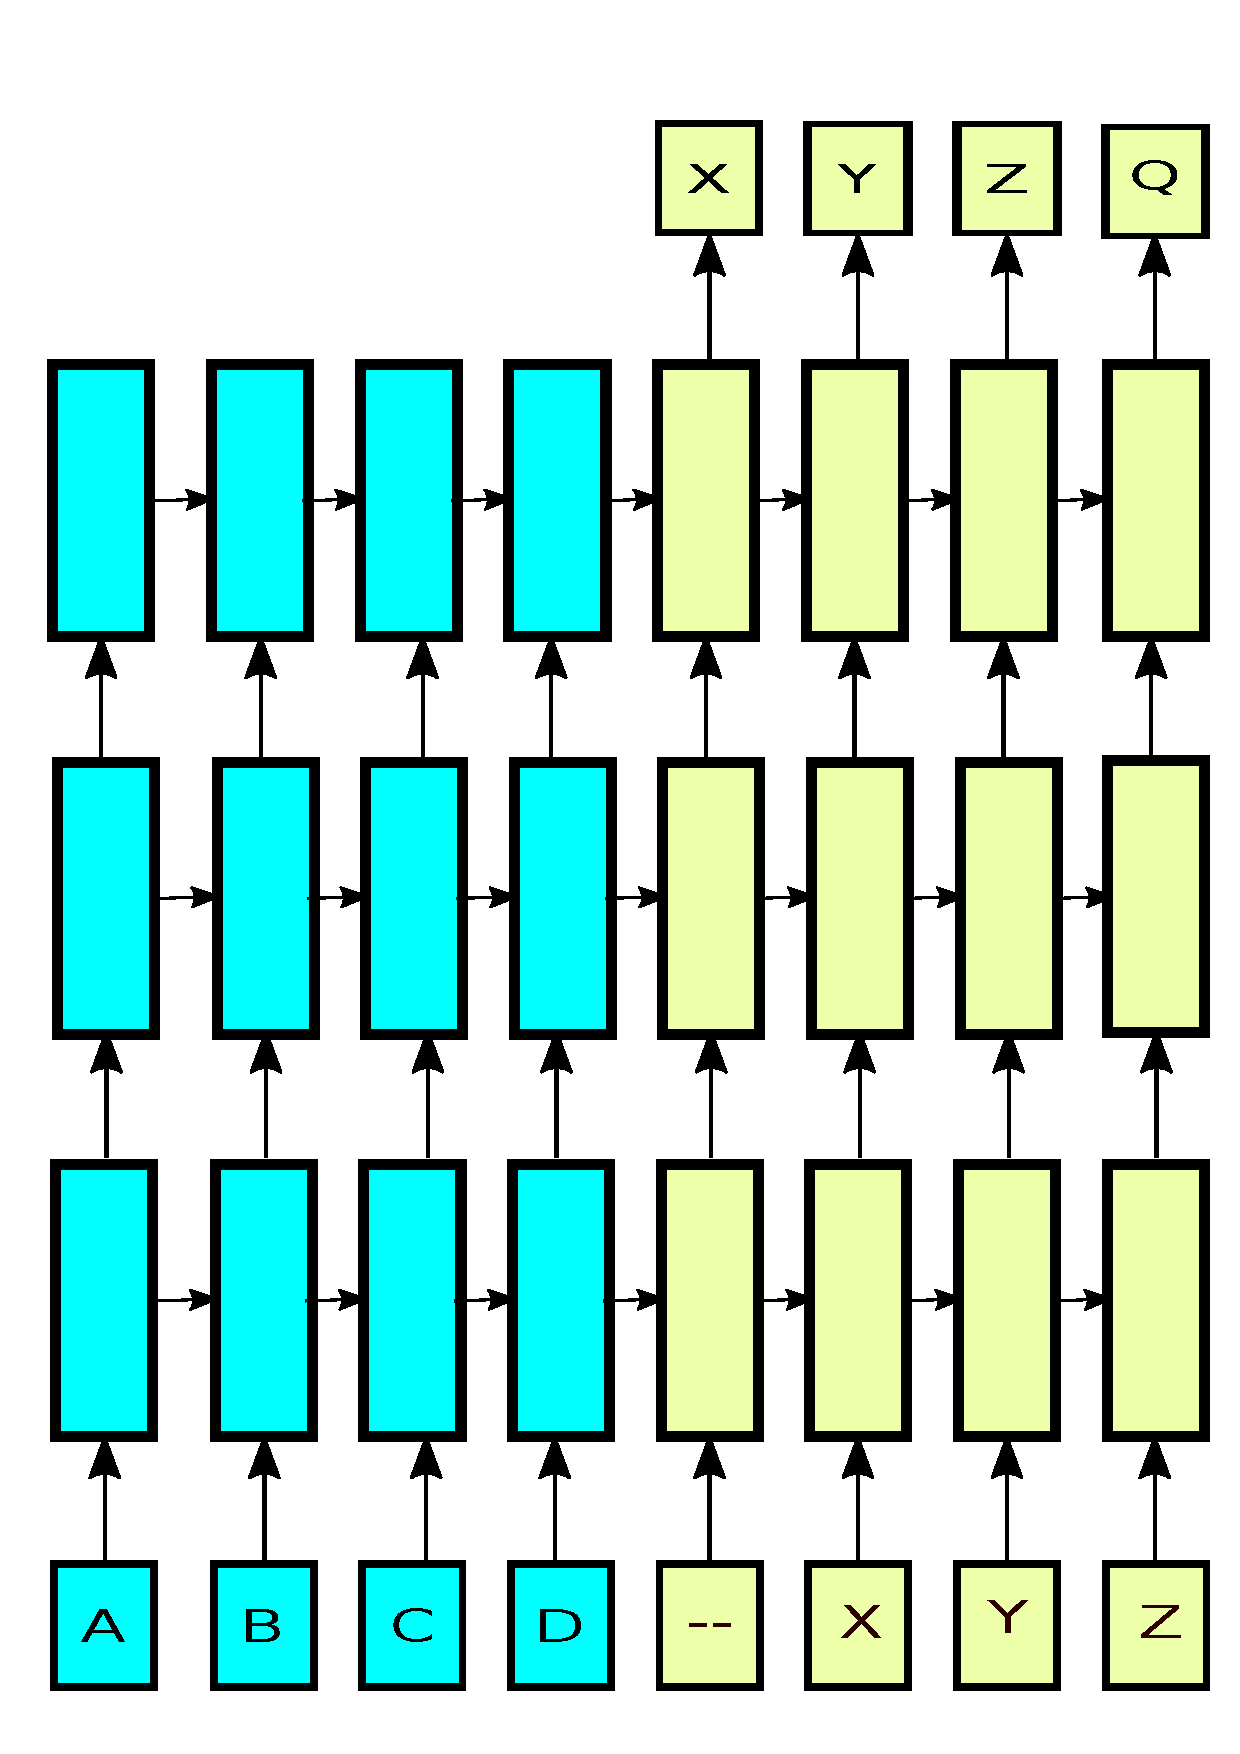
\includegraphics[width=.49\linewidth]{img/seq2seq_deep.pdf}
  \caption{A more powerfuls Sequence to sequence model}
  \label{fig:seqdeep}
\end{figure}


\begin{figure}
  \centering
  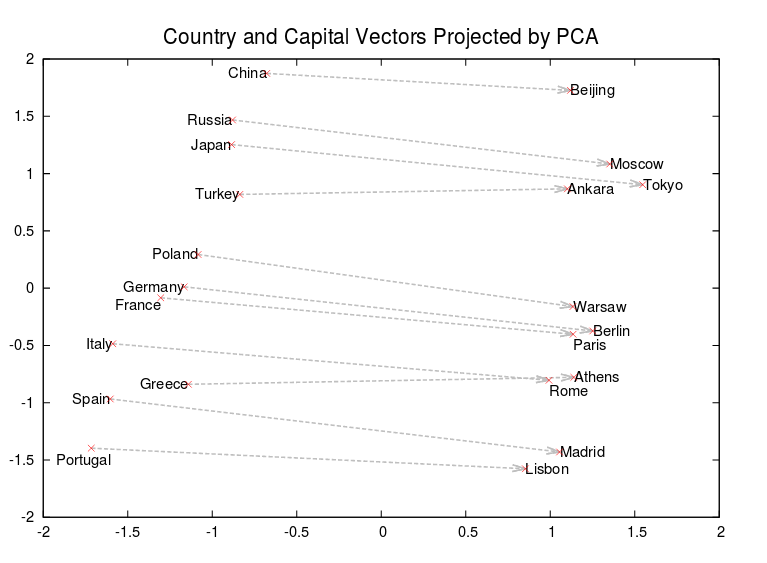
\includegraphics[width=.9\linewidth]{img/wordvec.png}
  \caption{
    Two-dimensional PCA projection of the 1000-dimensional word embedding.
  }
  \label{fig:wordvec}
\end{figure}


A simple  sequence to  sequence  model is  shown  in Fig.\ref{fig:seq}.  Just by
making  the model  more  deeper,  without  any  special  treatment  for  machine
translation, the paper  achieved state-of-the art results. The model is  trained
on WMT English to French  dataset with 12M sentences consisting  of  348M French
words and  304M English  words using  160,000 of the most frequent words for the
source language and  80,000 of the most  frequent words for the target language.
Every out-of-vocabulary word was replaced with a special \textbf{UNK} token. The
network has  4  LSTM layers with 1000 LSTM cells in each  layer. The  paper used
1000 dimensional word embedding  to  represent the words as vector following the
word2vec paper \cite{mikolov2013distributed}. word2vec formulated the problem of
learning word embedding as an energy maximization problem using a  simple neural
network  with just one  hidden layer.  The  energy  maximized is called Negative
sampling. The resulting vector embedding is empirically shown to have arithmetic
properties. i.e. $\,$France -  Paris +  Germany  is roughly  equal  to Berlin as
shown  in Fig.\ref{fig:wordvec}. The paper an impressive BLEU score of 33.3 even
without doing anything specific for machine translation.


\begin{figure}
  \centering
  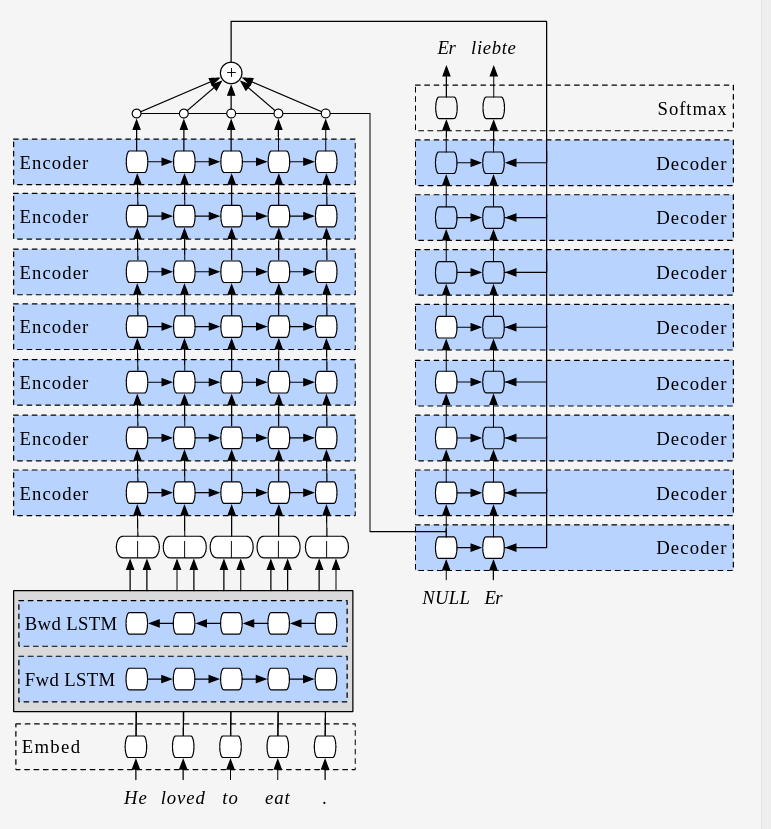
\includegraphics[width=.9\linewidth]{img/gnmt_1.png}
  \caption{The core architecture of GNMT }
  \label{fig:gnmt1}
\end{figure}


\begin{figure}
  \centering
  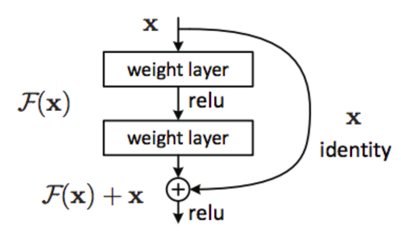
\includegraphics[width=.9\linewidth]{img/residual.png}
  \caption{Residual connections}
  \label{fig:residual}
\end{figure}


\begin{figure}
  \centering
  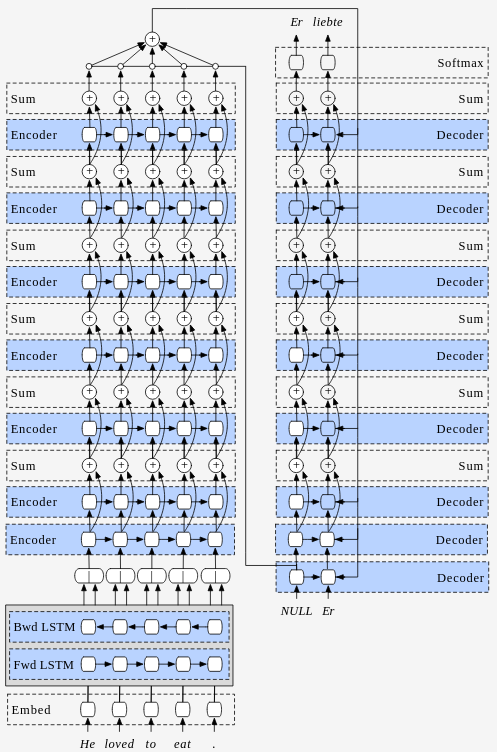
\includegraphics[width=.9\linewidth]{img/residual_gnmt.png}
  \caption{GNMT with residual connections}
  \label{fig:gnmtres}
\end{figure}


\subsection{Google Neural Machine System}

Most  likely  Google  runs  the   worlds  biggest  machine  translation  service
supporting 103  languages (at the time of writing this  article) serving about a
billion query  every day.  Google translate  team  published  a  detailed  paper
describing their  neural machine translation  system \cite{wu2016google}. In the
following section we will discuss  the key ideas  described  in the  paper. This
paper is very unique in the  sense that  it is much more than an academic paper.
The  paper explains  most  of the components of  the system including  a  lot of
engineering  details and also has  a lot of  components  that are inspired  from
other recent breakthroughs  in machine translation and deep learning research in
general. The basic architecture is heavily inspired by the jointly  learning  to
align and  translate \ref{sec:JT}  and  \ref{sec:seq}. The  core architecture is
shown in Fig.\ref{fig:gnmt1}. It combines the  idea of context with the a deeper
sequence to  sequence encoder-  decoder  model with bi-directional LSTM  in  the
initial  layers of  the encoder. Both  the  encoder  and decoder  contains eight
layer.   It  also   made   use  of   the  Residual   connections  introduced  in
\cite{he2016deep}.  Residual connection are helpful in alleviating the vanishing
gradients problem in  an interesting  manner as shown in Fig.\ref{fig:residual}.
In a DNN each  layer can be interpreted as transforming the  input  $x$ to a new
manifold  by learning $F (x)$ but in a residual network only learn the change to
be  applied to  the  input  ($x + F  (x)$). There  is  always  an  identity skip
connection between layers helping in the  constant gradient flow which otherwise
might vanish. The residual learning enables training very deep networks as shown
in Fig.\ref{fig:gnmtres}.

The author  also tried to use a enhanced cost  function. The usual cost function
maximized   by    the    training    process   is    the    maximum   likelihood
$$\mathbb{O}_{ML}(\Theta) = \sum_{i=1}^N  log  P_\Theta  (Y^{*(i)} | X^{(i)}) $$
but this does not directly correspond to the BLEU score. To improve the BLEU the
authors  proposed  the  following  cost function. $$  \mathbb{O}_{ML}(\Theta)  =
\sum_{i=1}^N  \sum_{Y=\mathbb{Y}}^N  log  P_\Theta  (Y^{*(i)}  |  X^{(i)})  r(Y,
Y^{*(i)} ) $$ where $r (\cdot)$ is per-sentence score computed as an expectation
over all $Y$ up to certain-length.

In terms  of the training  process, just one encoder and one decoder is used for
all  language pairs. The authors reported  several nice properties of the  joint
language training. One  highlight  is that this  enables zero-shot learning. The
system  is able  to translate  between  the  language pairs it never  saw in the
training data. Also  the languages for which huge training data does  not exists
benefited from the joint training. The  zero shot learning property is discussed
in  detail  the paper  \cite{johnson2016google}.  To enable a  single decoder to
generate target sentence for all the languages, the input text is  suffixed with
additional  tokes like $<\_\_EN\_\_>,  <\_\_FR\_\_>, <\_\_DE\_\_>, <\_\_ES\_\_>$
indicating the target language to be generated.

A  simple  sequence to sequence  model is shown in Fig.  \ref{fig:seq}.  Just by
making  the model more deeper as in Fig.  \ref{fig:seqdeep}, without any special
treatment for machine translation, the  paper achieved state-of-the art results.
The  model  as trained on  WMT English  to  French  dataset with  12M  sentences
consisting of 348M French words and 304M English words using 160,000 of the most
frequent words for the source language and 80,000 of the most frequent words for
the  target  language. Every out-of-vocabulary  word was replaced with a special
\textbf{UNK} token. The network has 4 LSTM layers with 1000  LSTM cells in  each
layer. The paper used 1000 dimensional word embedding  to represent the words as
vector  following  the  word2vec paper  \cite{mikolov2013distributed}.  Word2vec
formulated  the  problem of  learning word embedding  as an energy  maximization
problem using a simple neural  network  with just one  hidden  layer. The energy
maximized is  called  Negative  sampling.  The  resulting  vector  embedding  is
empirically shown  to  have arithmetic  properties.  i.e.  $\,$France -  Paris +
Germany is roughly equal to Berlin as shown in Fig. \ref{fig:wordvec}. The paper
an  impressive BLEU score  of  33.3 even  without  doing  anything  specific for
machine translation.

One another interesting aspect of the GNMT is the use  of Quantizable  Model and
Quantized  Inference.  Since GNMT has to  serve  a  huge volume of users  in the
production,  the service is  very computationally intensive  making hard for low
latency translation difficult.  Quantized Inference is  the process of using low
precession  arithmetic operations during  the inference. The idea of  using  low
precession arithmetic  got  inference has  been  tried  since  the early days of
neural  networks.  In  the recent  years, the  authors in \cite{wu2016quantized}
successfully demonstrated that a CNN training can  be sped up by a factor of 4-6
with minimal  loss  of accuracy in  the classification task. More  interestingly
\cite{li2016ternary} showed that weights of the neural networks can be quantized
to just three states, -1,0,1. But most of these success were restricted to CNNs.
In the paper GNMT  team  did the same  of RNNs. To  achieve this, the model were
constrained  during  training time. The nature of LSTMs remembering state across
multiple time steps posts additional challenges  in quantizing RNNs.  he forward
computation  of  an LSTM  stack with  residual connections  is modified  to  the
following:


\begin{equation}
  \begin{split}
    c^{'i}_t,m^i_t & = LSTM_i(c^{i}_{t-1},m^i_{t-1}, x^{i-1}_t; W^i ) \\
    c^{i}_t & = max(-\delta, min (\delta,c^{'i}_t )) \\
    x^{'i}_t & = m^{i}_t + x^{i-1}_t \\
    x^{i}_t & =  max(-\delta, min (\delta,x^{'i}_t )) \\
    c^{'i}_t,m^i_t & = LSTM_{i+1}(c^{i+1}_{t-1},
                       m^{i+1}_{t-1}, x^{i}_t; W^{i+1} ) \\
    c^{i+1}_t & =  max(-\delta, min (\delta,c^{'i+1}_t ))
  \end{split}
\end{equation}


and for keeping notation simple we drop the superscript $i$  and expand  further
as,


\begin{equation}
  \begin{split}
    W & = [W_1,W_2....W_8] \\
    i_t & =  sigmoid(W_1x_t + W_2m_t) \\
    {i'}_t & = tanh(W_3x_t + W_4m_t) \\
    f_t & =  sigmoid(W_5x_t + W_6m_t) \\
    o_t & = sigmoid(W_7x_t + W_8m_t) \\
    c_t & =  c_{t-1} \odot f_t + i^{'}_t \odot i_t \\
    m_t & = c_t \odot o_t
  \end{split}
\end{equation}


All the operations in the above equations are performed only with fixed point  8
bit or 16 bit integer multiplications.


\subsection{A Convolutional Encoder Model for NMT}

Despite all the success that recurrent neural  netowrks  have achieved in neural
machine translation, they have some shortcomings which makes them less appealing
for such a task. Recurrent neural networks have an inherently serial  structure,
meaning that their  camputations  cannot  be  fully parallelized. This contrasts
with  other types of networks, specifically covolutioanl neural  networks, which
operate  over a  fixed-size input sequence enabling simultaneous computation  of
all the features. Furthermore  recurrent  neural networks need  to traverse  the
full distance of  the serial  path  between  two features  to reach from one  to
another. This characteristics  leads  to  higher  difficulty  of  training these
models. Once  again  this  is  not  the  case  for some  other  models  such  as
convolutional neural networks in  which  a succession  of  convolutional  layers
provide shroter  path  between features.  \cite{DBLP:journals/corr/GehringAGD16}
Such  desired characteristics  of convolutional neural networks have resulted in
the recent trend to exploit their power in neural machine  translations. In this
and next sections we review a number of propsed techniques.


\begin{figure}
  \center
  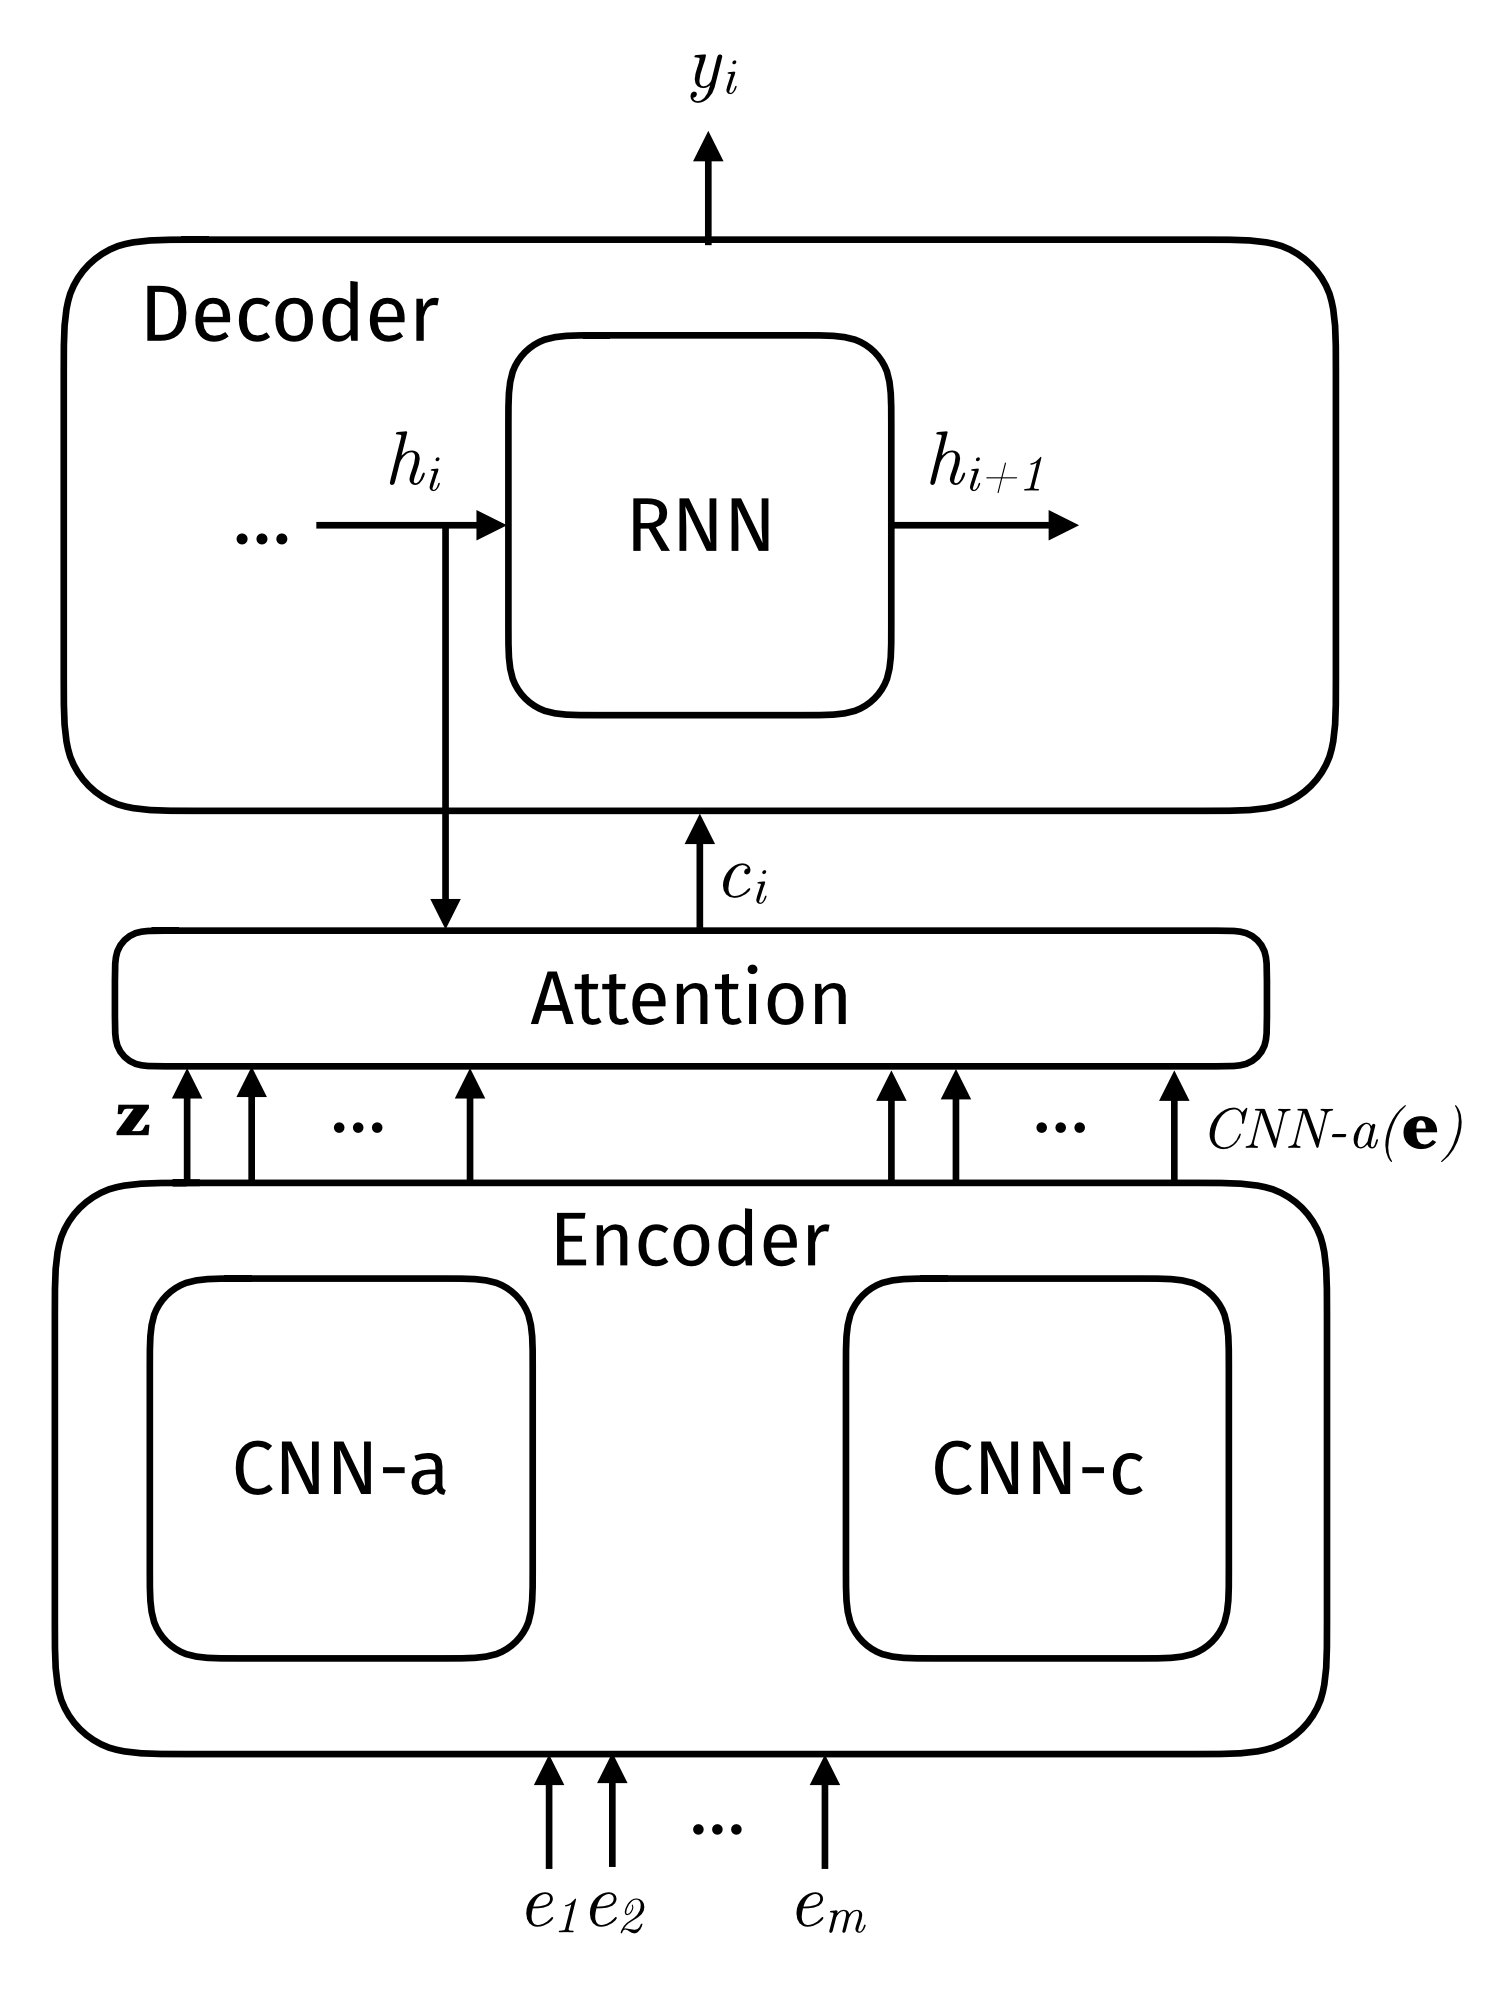
\includegraphics[width=0.5\textwidth]{img/CE}
  \caption{The architecture of convolutional encoder model}
  \label{fig:convenc}
\end{figure}


\citet{DBLP:journals/corr/GehringAGD16}   proposes   an   encoder-decoder  model
similar to that of \cite{bahdanau2014neural} in which the encoder is replaced by
a convolutional neural network. In this model, as  in \cite{bahdanau2014neural},
the  decoder is  a long  short-term memory recurrent  neural  network,  and  the
encoder  consists of  two one-dimensional convolutional  networks:  One  network
(CNN-a) generates  a  sequence containing  the encoded information about  fixed-
sized contexts (of kernel size), and the other (CNN-c) computes the  conditional
input for  the soft-attention mechanism  connecting the encoder and the decoder.
Fig. \ref{fig:convenc} schematically illustrates this architecture.

The  convolutional  networks  in  the encoder only contain convolutional  layers
without any pooling layer. This allows  the full input  sequence  length to  the
encoder  to be  retained. Moreover stacking multiple convolutional layers on top
of each other can increase the context width for each input  token  of the input
sequence.

As  convolutional layers do all their  calculations  in  parallel  and therefore
cannot distinguish  position of  the input  tockens, it is  necessary to somehow
encode the positional information in the input sequence before feeding it to the
encoder. To this end, \citet{DBLP:journals/corr/GehringAGD16} proposes to feed a
sequence $e_1, e_2, ..., e_m$ to the ecoder in which,


\begin{equation*}
  e_i = w_i + l_i
\end{equation*}


where  $w_i$  is a word embedding on the vocabulary of the source  language  and
$l_i$ is a positional embedding of the words of the source sentence.

The decoder  aims to capture a  distribution over the possible target vocabulary
by  transforming its LSTM  hidden  state  $h_i$ via a linear layer  with weights
$W_o$ and bias $b_o$,


\begin{equation*}
  p(y_{i+1} \vert y_1, ..., y_i, \textbf{x}) =
  \text{softmax}(W_o h_{i + 1} + b_o)
\end{equation*}


The  conditional input $c_i$ to the  LSTM is  computed via  a simple dot-product
soft-attention  mechanism,  i.e. a  dot-product  between  the set of  calculated
attention weights and the  sequence coming form CNN-c. In order to calculate the
attention  scores, first the  hidden  state  $h_i$  is  transformed  by a linear
transformation  with weights  $W_d$  and bias  $b_d$  to match  the  size  of an
embedding  of the  previous  target word $g_i$ and then it  is summed  with that
embedding. Then  this vector is used to calculate the each attention score via a
softmax over the  product  of all  these neworks and  the  sequence comming from
CNN-a:


\begin{align*}
  d_i &= W_d h_i + b_d + g_i \\
  z_i &= \text{CNN-a}(e_i) \\
  c_i &= \sum_{j = 1}^{T}{a_{ij}\text{CNN-c}(e_j)} \\
  a_{ij} &= \frac{exp(d_i^T z_j)}{\sum_{t = 1}^{m}{exp(d_i^T z_t)}}
\end{align*}


The experimental results show that this architecture's performance is comparable
to that of bi-directional recurrent  neural networks while  achieving two  times
speed up in generation of target translation. Table \ref{tab:convseqblue}  lists
the BLEU score achieved by this model for a few datesets.


\begin{table}
  \center
  \begin{tabular}{lrrr}
  \hline
    Encoder & WMT'16 en-ro & WMT'15 en-de & WMT'14 en-fr \\
  \hline
    BiLSTM & 27.4 & 23.2 & 34.6 \\
    Convolutional & 27.8 & 24.3 & 35.7 \\
  \hline
  \end{tabular}
  \caption{Performance  comparison of  convolutional  encoder  model  with a bi-
  directional neural network in terms of BLEU score}
  \label{tab:convseqblue}
\end{table}


Another interesting observation is that in recurrent neural networks the learned
attention scores are sharp but do not necessarily represent a correct alignment,
while for convolutional encoders the  scores are less focused but still indicate
an approximate source  location.  Fig.  \ref{fig:atts}  illustrates  the learned
attention scores  for a  sentence from WMT'15 English-German translation using a
2-layer  BiLSTM  and  a convolutional  encoder with  15-layer CNN-a  and 5-layer
CNN-c.


\begin{figure}
  \center
  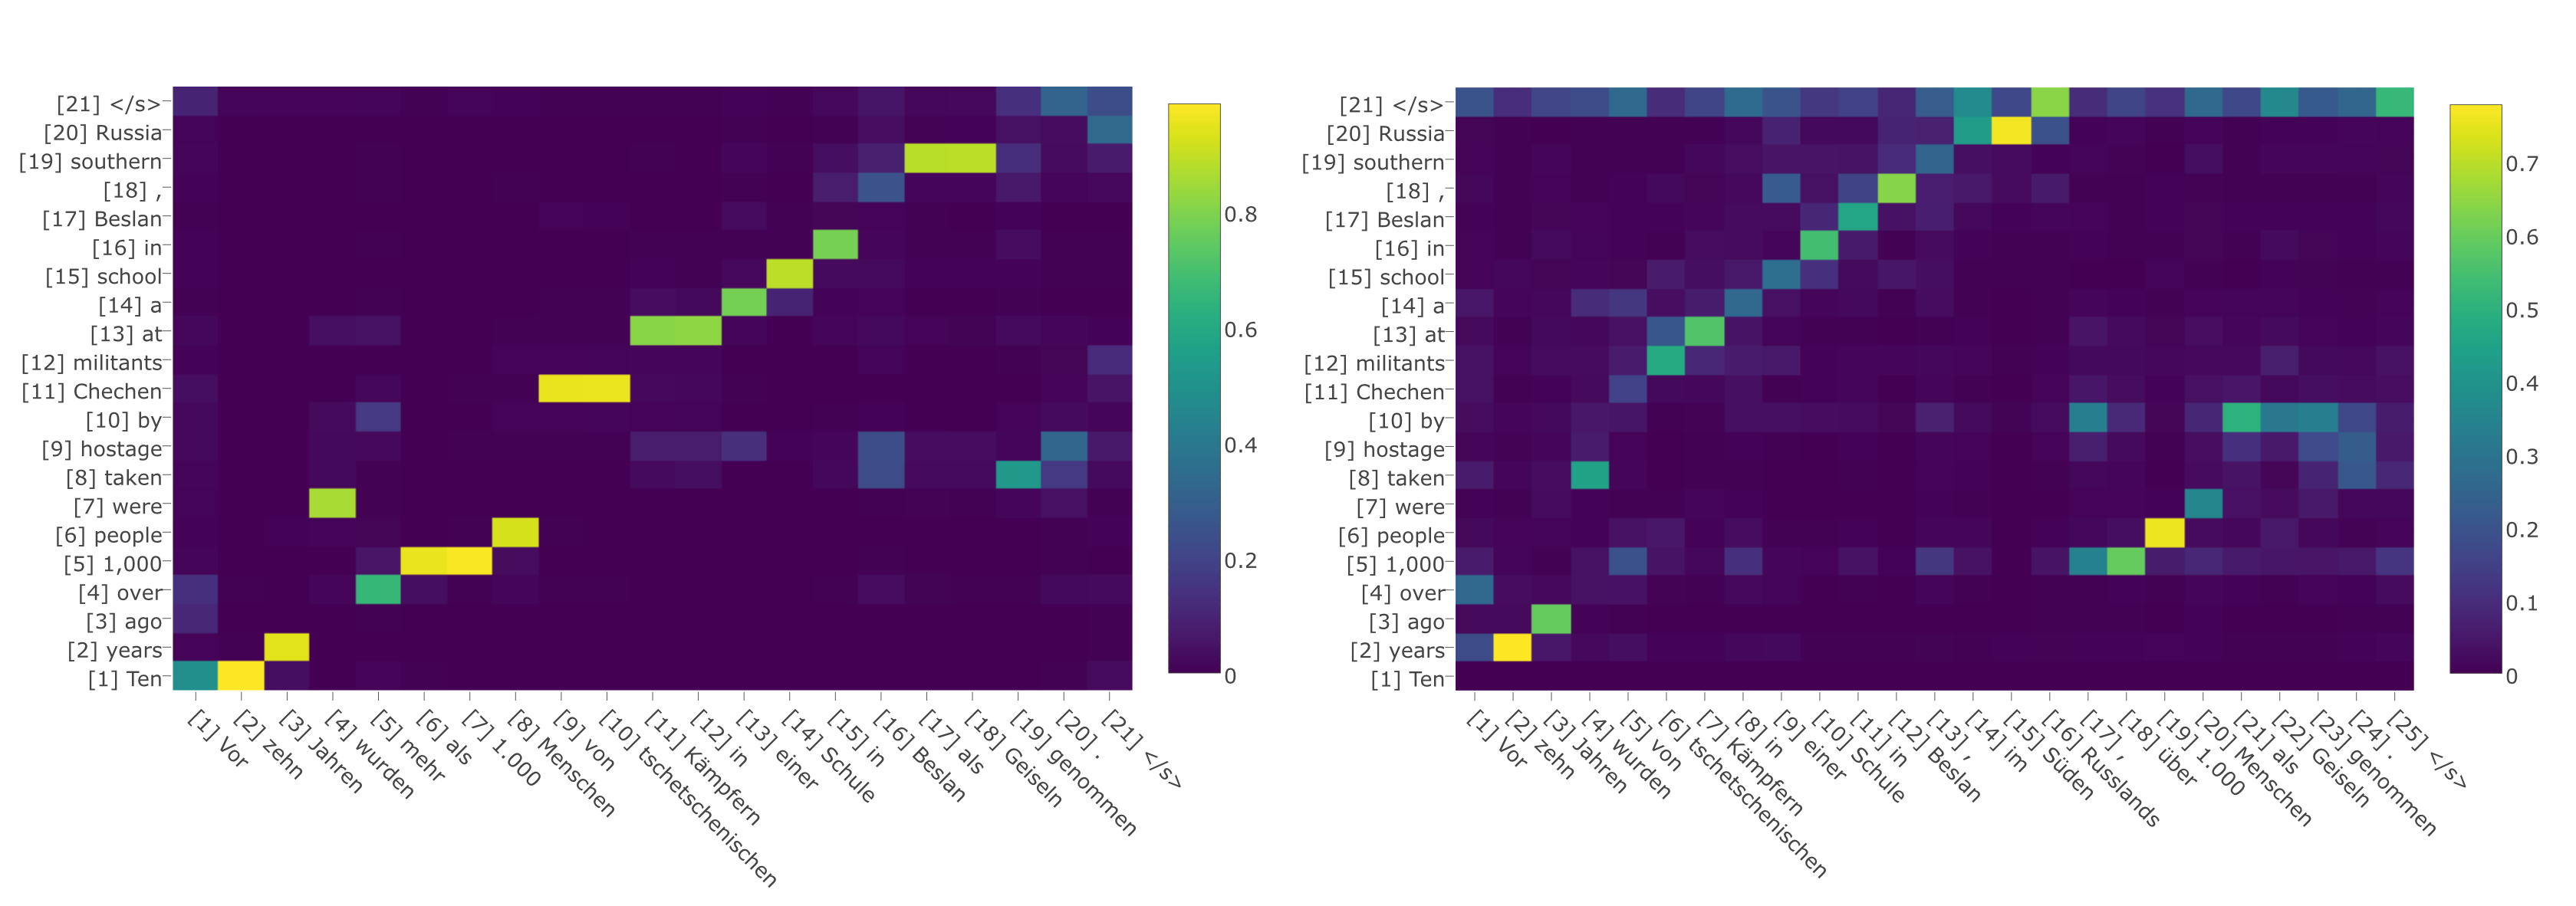
\includegraphics[width=\textwidth]{img/atts}
  \caption{Attention scores  for  a  BiLSTM  (top) and a  convolutional  encoder
  (bottom)}
  \label{fig:atts}
\end{figure}


\subsection{Convolutional Sequence to Sequence Learning}

Based                 on                 \cite{DBLP:journals/corr/GehringAGD16},
\citet{DBLP:journals/corr/GehringAGYD17}   further   developed   the   idea   of
convolutional  encoders and  introduced  a  fully convolutional  encoder-decoder
architecture. In this model  both  encoder  and decoder networks  share a simple
convolution block structure  that computes  intermediate states based on a fixed
number  of input elements.  Each block consists of a one-dimensional convolution
followed by  a non-linearity. Once  again the relationship between distant words
in the input sequence is captured by stacking multiple such blocks on top of one
another, and non-linearities in the  blocks  allow the  network to  exploit this
full   input   field,   or   to    focus   on   fewer   elements    if   needed.
\citet{DBLP:journals/corr/GehringAGYD17}  proposes the use of gated linear units
(GLU) as non-linearity.

Each  convolution kernel  of size $k$ is  parameterized as  $W \in \R^{2d \times
kd}$, $b_w \in \R^{2d}$  and takes as input $X \in  \R^{k \times d}$  which is a
concatenation of  $k$ input elements embedded in $d$ dimensions and maps them to
a single element $Y = [A B] \in \R^{2d}$. Then applying a gated linear unit non-
linearity $v([A B]) = A  \otimes \sigma(B)$ where $A, B \in  \R^d$ and $\otimes$
is point-wise  multiplicaiton, results in a single output element  of  size $d$.
Subsequent  layers  operate  in the  same manner  over  $k$ such  elements  from
previous layer. Fig.  \ref{fig:convseq2seq} illustrates the architecture  of the
model.


\begin{figure}
  \center
  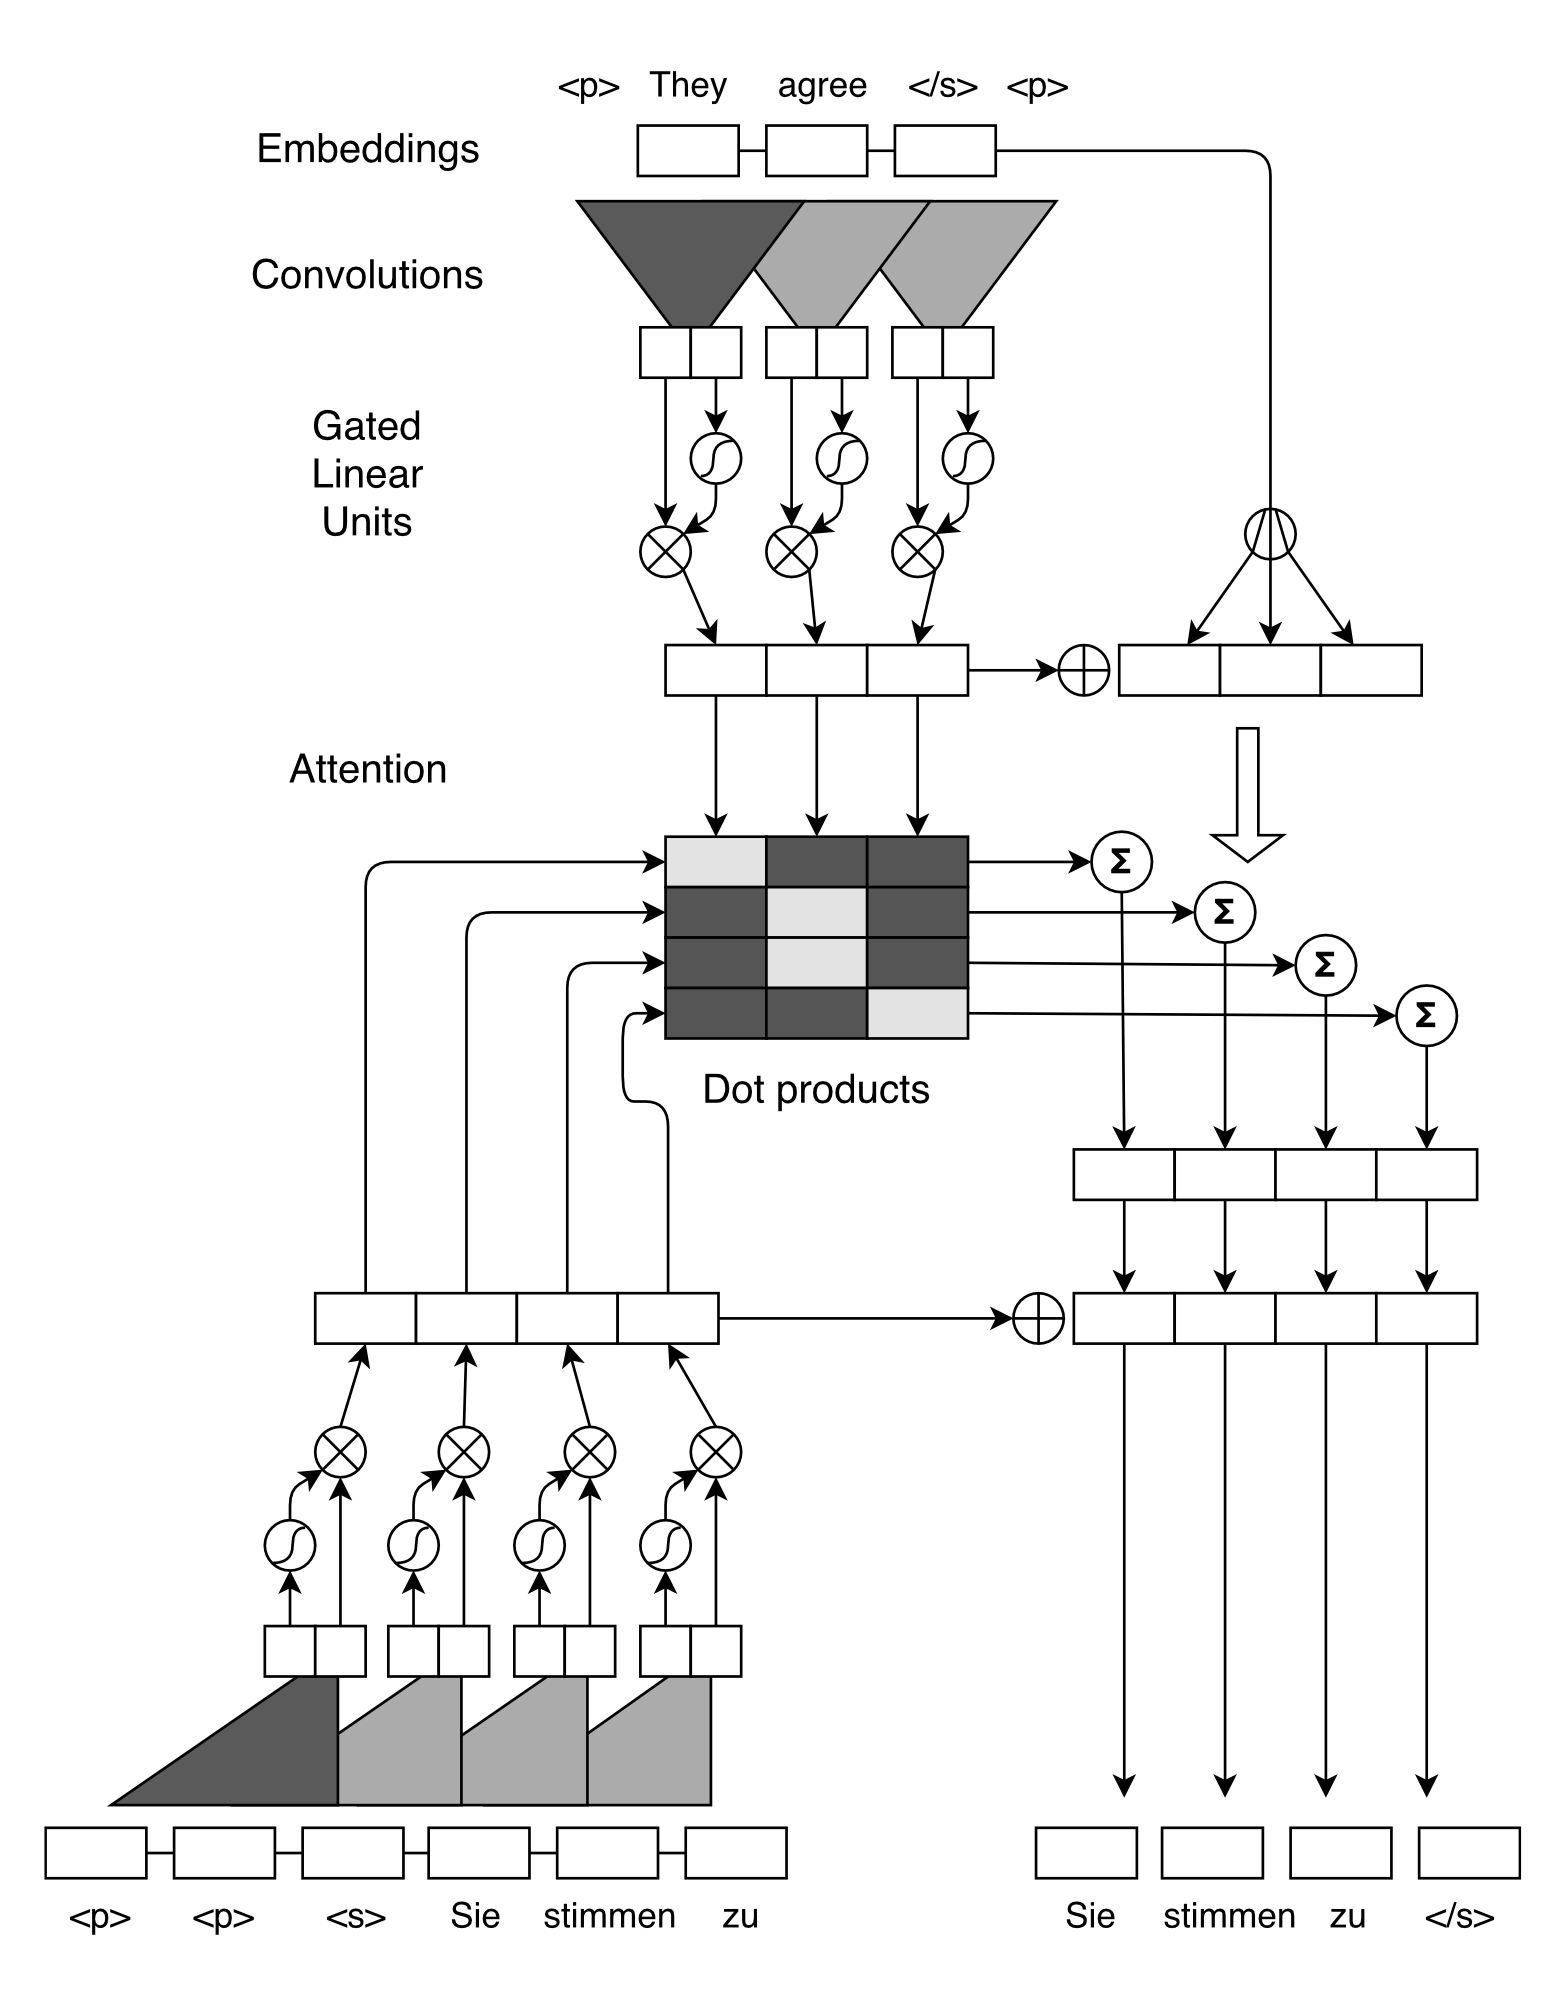
\includegraphics[width=0.6\textwidth]{img/CS2S}
  \caption{Architecture of convolutional sequence to sequence learning.}
  \label{fig:convseq2seq}
\end{figure}


Another  introduced  improvement over  previous model is multi-step attention in
which a set of different conditional inputs are calculated for each layer of the
decoder. To compute the attention,  the current  hidden  state $h^l_i$ of $l$-th
layer of decoder  is combined with an  embedding of the previous target  element
$g_i$. Once  the conditional input $c_i^l$ has been computed, it is simply added
to the output of the corresponding layer $h^l_i$.


\begin{align*}
  y_i^l &= h_i^l + c_i^l \\
  c_i^l &= \sum_{j = 1}^{m}{a_{ij}^l (z_j^u + e_j)} \\
  a_{ij}^l &= \frac{exp (d_i^l \cdot z_j^u)}
  {\sum_{t = 1}^{m}{exp (d_i^l \cdot z_t^u)}} \\
  d_i^l &= W_d^l h_i^l + b_d^l + g_i
\end{align*}


Experimental results show that this translation model achieves similar or higher
BLEU scores  as that of GNMT while bringing almost an order of magnitude seep up
in translation generation. Table \ref{tab:convseq2seqbleu} lists the  BLEU score
achieved by this model for a few datesets.


\begin{table}
  \center
  \begin{tabular}{lrrr}
  \hline
    Model & WMT'16 en-ro & WMT'15 en-de & WMT'14 en-fr \\
  \hline
    GNMT & - & 24.61 & 39.92 \\
    ConvS2S & 29.88 & 25.16 & 40.46 \\
  \hline
  \end{tabular}
  \caption{Performance  comparison of convolutional  sequence to  sequence model
  with GNMT in terms of BLEU score}
  \label{tab:convseq2seqbleu}
\end{table}


\subsection{Depthwise Separable Convolutions for NMT}

Another     convolution-based      translation      model     is     due      to
\citet{DBLP:journals/corr/KaiserGC17}. Even though convolutions unlike recurrent
neural networks can provide an efficient non-local referencing across time, they
still  suffer   from  computational   complexity  and   large  parameter  count.
\cite{DBLP:journals/corr/KaiserGC17} Addresses this issue by introducing a model
based upon  so-called  depthwise  separable  convolutions.  Depthwise  Separable
Convolution  consists of a depthwise convolution, i.e an operator which performs
a spatial convolution independently over each  channel of the input, followed by
a pointwise convolution, i.e. a regular $1 \times 1$ convolution.

The rationale behind this definition  is  the  expermentally-verified assumption
that the  2D and 3D inputs that convolutions operate on will feature both fairly
independent    channels    and    highly    correlated     spatial     locations
\cite{DBLP:journals/corr/KaiserGC17}.  As  a  result one  can  simplify  regular
convolution's  feature  learning over  a joint "space-cross-channels realm" into
two  simpler  steps,  i.e.  a  spatial  feature  learning  step,  and a  channel
combination  step, while  reducing  the  number  of  parameters.  More  formally
depthwise separable convolution can be written as follows:


\begin{align*}
  Conv (W, y)_{i,j} &= \sum_{k,l,m}^{K,L,M}{W_{k,l,m} \cdot y_{i+k,j+l,m}} \\
  PointwiseConv (W, y)_{i,j} &= \sum_{m}^{M}{W_m \cdot y_{i,j,m}} \\
  DepthwiseConv (W, y)_{i,j} &= \sum_{k,l}^{K,L}{W_{k,l} \cdot y_{i+k,j+l}} \\
  SepConv (W_p, W_d, y)_{i,j} &=
    PointwiseConv_{i,j}(W_p, DepthwiseConv_{i,j}(W_d, y))
\end{align*}


Table \ref{tab:convpar} lists the number fo parameters for a regular convolution
as well as a depthwise separable  convolution with  $c$ channels and filters and
one-dimensional kernel  of  size $k$. As it can be seen  for larger kernel sizes
the number  of  parameters in  depthwise separable convolution  is significantly
less than regular convolutions.


\begin{table}
  \center
  \begin{tabular}{lr}
  \hline
    Convolution & Number of parameters\\
  \hline
    Conv & $k \cdot c^2$ \\
    SepConv & $k \cdot c + c^2$ \\
  \hline
  \end{tabular}
  \caption{Number of parameters in convolution operations}
  \label{tab:convpar}
\end{table}


The SliceNet  model  introduced  in \cite{DBLP:journals/corr/KaiserGC17},  has a
similar structure  to other encoder-decoder models. It  first embeds the  inputs
and outputs by two independent networks  and concatenates them and the feeds the
result  into  a  decoder. At  each  step,  the  decoder produces  a  new  output
prediction given the  encoded inputs and the encoding of the previously produces
outputs. Fig. \ref{fig:sn} illustrates the architecture of SliceNet model.


\begin{figure}
  \center
  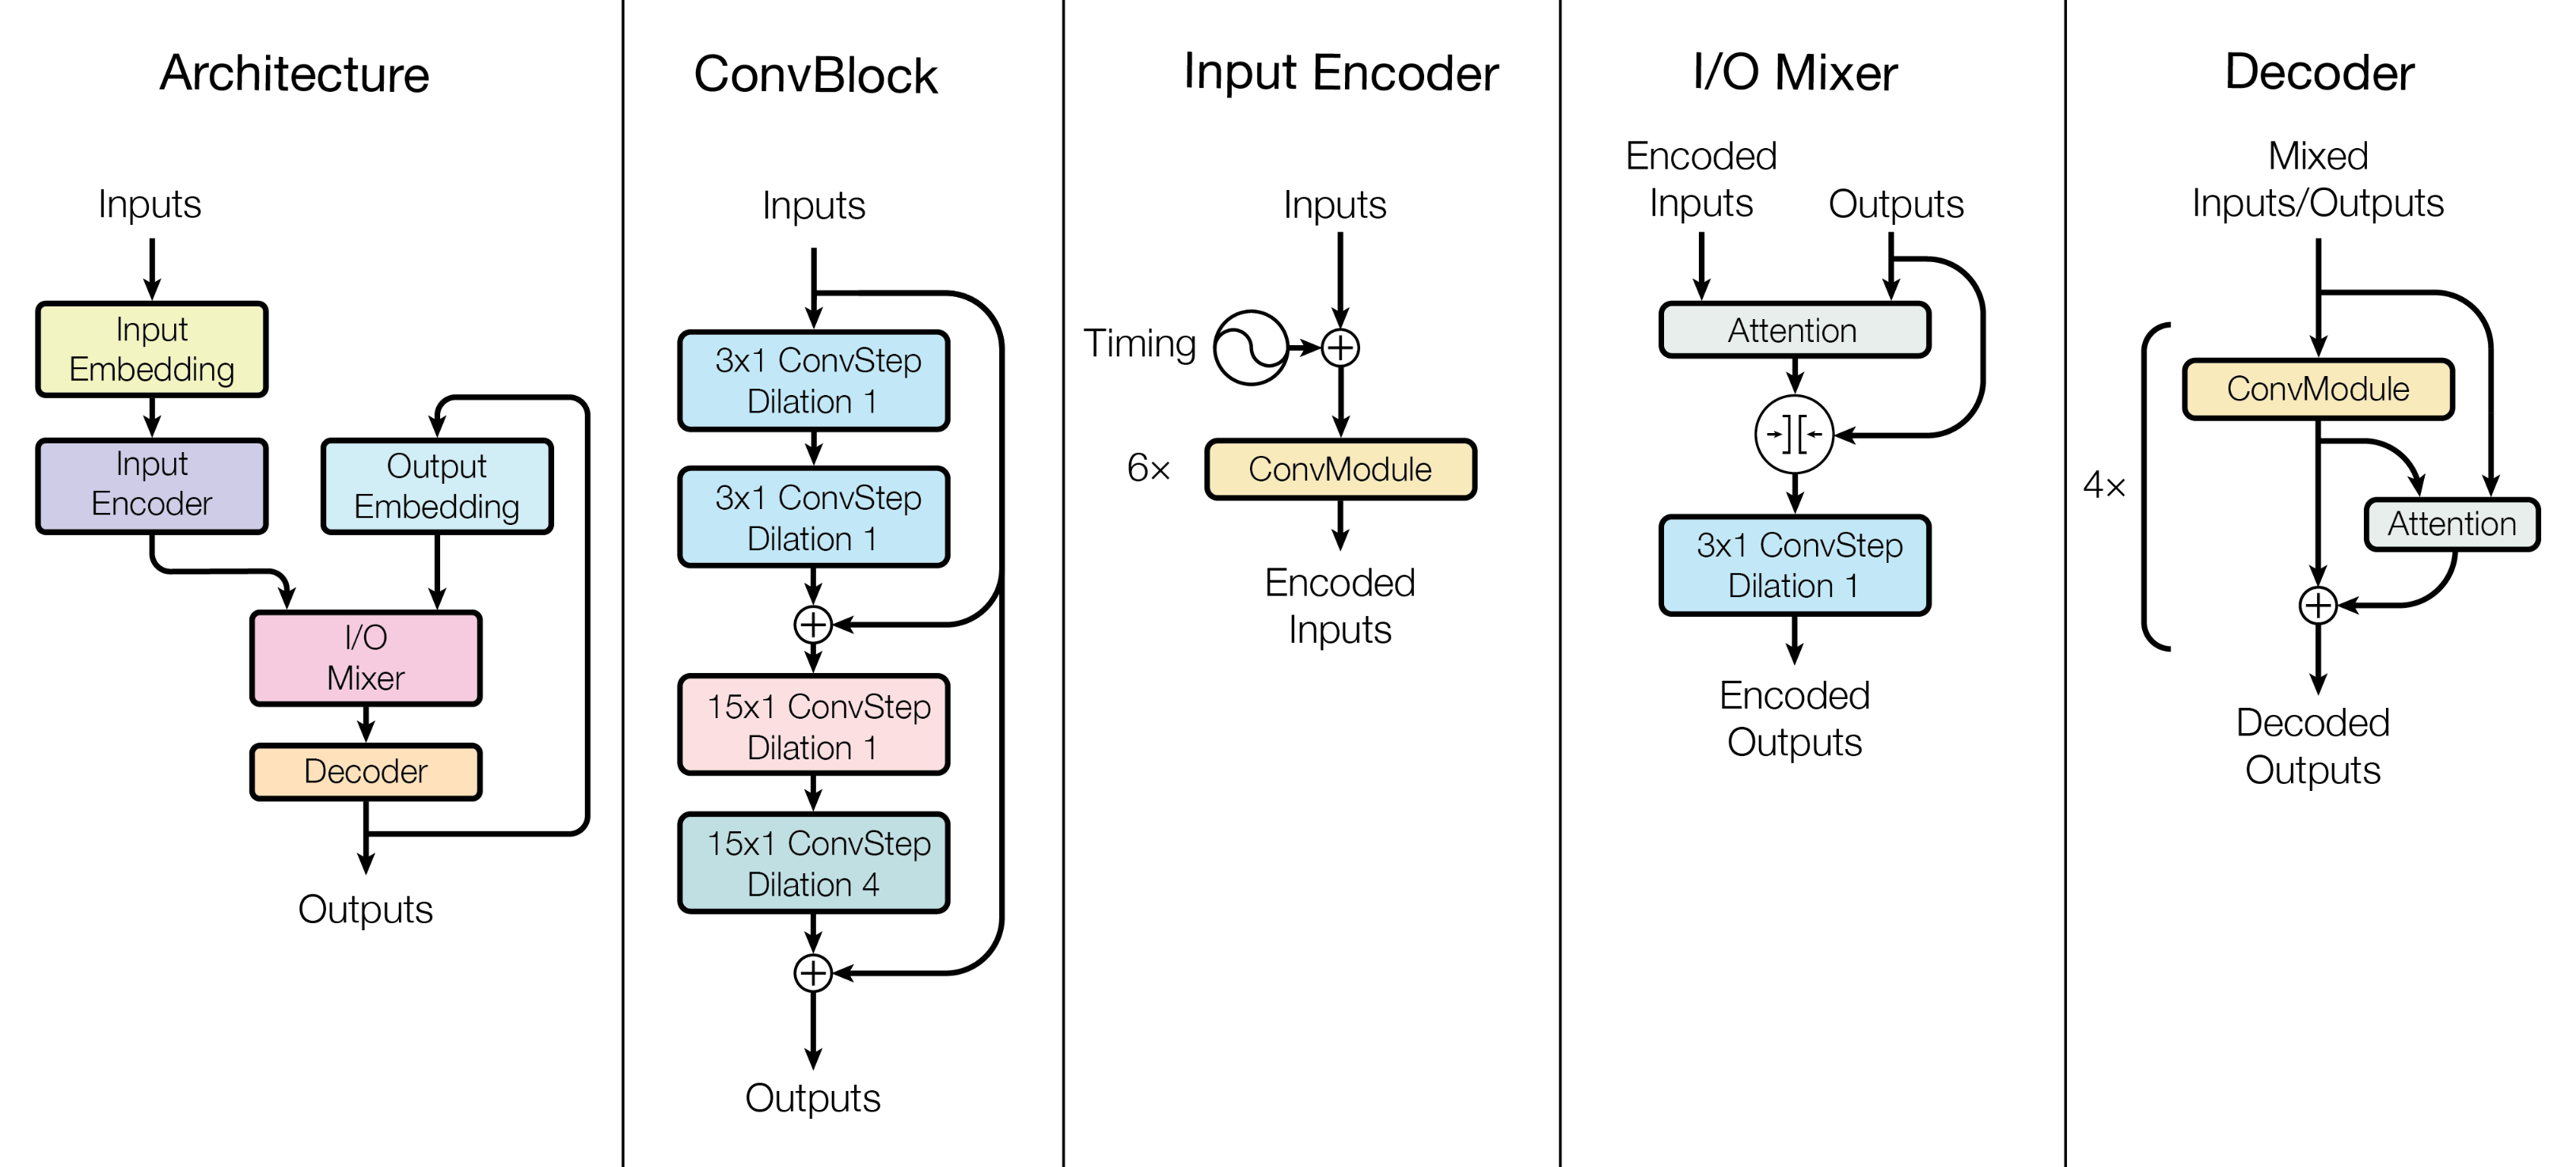
\includegraphics[width=\textwidth]{img/SN}
  \caption{The architecture of SliceNet}
  \label{fig:sn}
\end{figure}


The convolution modules in  SliceNet  use rectified linear units  (ReLU) as non-
linearities. Besides the ReLU activations are followed by a normalization layer.
Therefore a complete convolution module is defined as,


\begin{align*}
  ConvStep_{d,s}(W, x) &= LN (SepConv_{d,s}(W, ReLU (x))) \\
  LN (x) &= \frac{G}{\sigma (x)}(x - \mu (x)) + B
\end{align*}


In order to encode the  positional information, SliceNet  add a so-called timing
signal to the input sequence. This signal is defined as follows,


\begin{align*}
  timing (t, 2d) &= sin (t/1000^{2d/depth}) \\
  timing (t, 2d + 1) &= cos (t/1000^{2d/depth})
\end{align*}


For  given  source of shape $[m,  depth]$  and target  of shape $[n, depth]$ the
attention mechanism used in SliceNet computes the feature vector similarities at
each position and re-scales according to the depth,


\begin{align*}
  attention(source, target) &= \\
  Attend(source, &ConvStep_{4,1}((W_a1^{5 \times 1}, attention1(target))))
\end{align*}


\begin{align*}
  attention1(x) &= ConvStep_{1,1}(W_a1^{5 \times 1} \cdot x + timing) \\
  Attend(source, target) &= \frac{1}{\sqrt{depth}} \cdot
    softmax(target \cdot source^T) \cdot source
\end{align*}


The experimental results presented in \cite{DBLP:journals/corr/KaiserGC17} shows
that  SliceNet  improves  the  BLEU  score  in  comparison  to  both   GNMT  and
convolutional sequence to sequence models. Table \ref{tab:snbleu} lists the BLEU
scores for one dateset.


\begin{table}
  \center
  \begin{tabular}{lr}
  \hline
    Model & newstest 14 \\
  \hline
    GNMT & 24.6 \\
    ConvS2S & 25.1 \\
    SliceNet & 26.1 \\
  \hline
  \end{tabular}
  \caption{Performance comparison of SliceNet with other models in terms of BLEU
  score}
  \label{tab:snbleu}
\end{table}


\bibliographystyle{plainnat}
\bibliography{literature}


\end{document}
